\documentclass[a4paper,12pt]{book}
\usepackage[utf8]{inputenc}
\usepackage{graphicx}
\usepackage{tikz}
\usepackage{wasysym}
\usepackage{hyperref}

\usepackage{array}
\newcolumntype{L}[1]{>{\raggedright\let\newline\\\arraybackslash\hspace{0pt}}m{#1}}
\newcolumntype{C}[1]{>{\centering\let\newline\\\arraybackslash\hspace{0pt}}m{#1}}
\newcolumntype{R}[1]{>{\raggedleft\let\newline\\\arraybackslash\hspace{0pt}}m{#1}}

\newcommand{\SourceCodeScale}{0.5}
\newcommand{\FigureScale}{0.4}

\hypersetup{
	colorlinks=true, % make the links colored
	linkcolor=blue, % color TOC links in blue
	urlcolor=red, % color URLs in red
	linktoc=all % 'all' will create links for everything in the TOC
}

\begin{document}


\author{Fakhir Shaheen}
\title{Android Development \\ A Practical Approach}
\date{September 2016}

\frontmatter
\maketitle
\tableofcontents

\mainmatter



%%%%%%%%%%%%%%%%%%%%%%%%%%%%%%%%%%%%%%%%%%%%%%%%%%%%%%%%
%% Preface


\chapter{Introduction}

... Add some stuff here ...
\chapter{Tour of Android Studio}

\section{Creating Android Project}
When you launch android studio for the first time, it will show you the welcome Welcome. (If you do not see the dialog, you may have created projects before. In that case, choose File $\rightarrow$ New Project). Following figure shows the welcome screen:

\begin{center}
	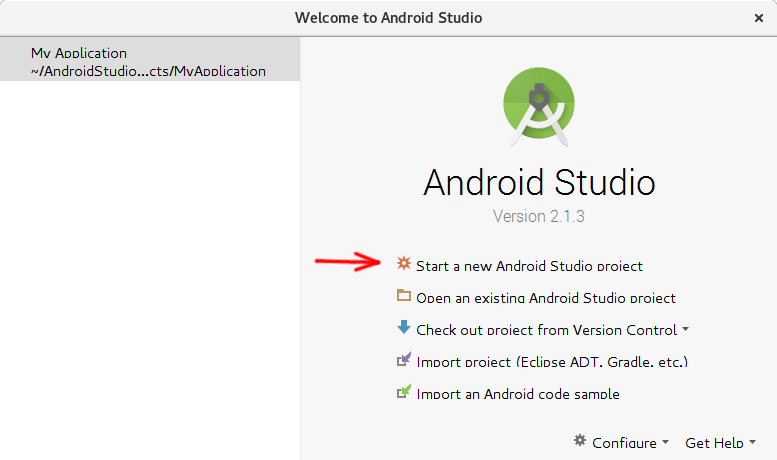
\includegraphics[scale=0.3]{chapters/ch02/images/1_welcome_screen}
\end{center}

The left side panel lists the projects that you've already created. The right side panel contains a bunch of buttons and options. You can import projects or open legacy code through here. At the bottom of this window, there is a configure button with a ``cog'' icon. Clicking it brings a drop down menu from where you can install or update various features and plugins. For now we will skip it.

From the right side panel, click on ``Start a new Android Studio project'' option (marked by the red arrow). This will take you to the configuration screen shown below:

\begin{center}
	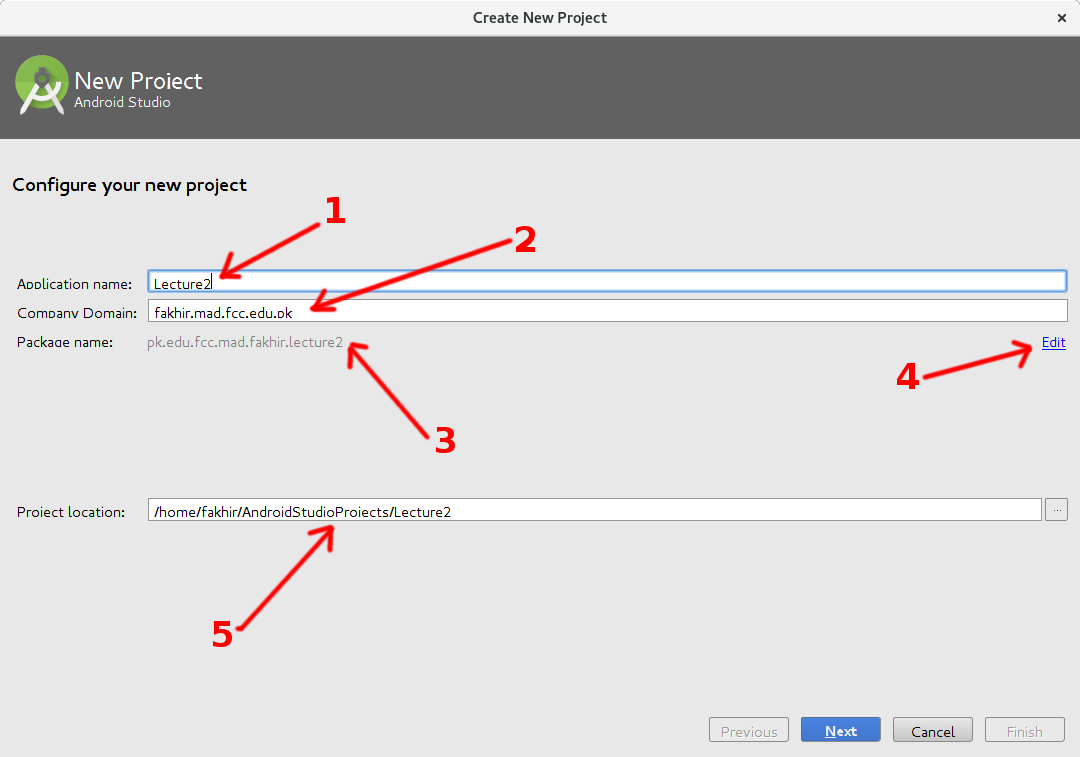
\includegraphics[scale=0.3]{chapters/ch02/images/2_app_name}
\end{center}

Each of the numbered arrows are explained in the list below:

\begin{enumerate}
	\item \textit{Application name:} This is the name of your application. You can change it to anything you like. For this exercise let's rename it to ``Lecture 2''.
	\item \textit{Company Domain:} This is a global identifier that will uniquely identify you app. This has to be different from all of the apps currently available on the android app store (or google play store). You can put it any valid string as long as it is unique.
	\item \textit{Package name:} Android studio automatically generates a string according to the previously entered information. You might've seen similar structure when programming for Java language.
	\item \textit{Edit:} If you need to give your own package name, then just click on ``Edit'' at the right side. We will leave the default value for now.
	\item \textit{Project location:} The complete path of the current project. You can change it if you like, but again we will leave the default value.
\end{enumerate}

Click next to go to the ``Target Android Devices'' screen. That'll bring you to the following window:

\begin{center}
	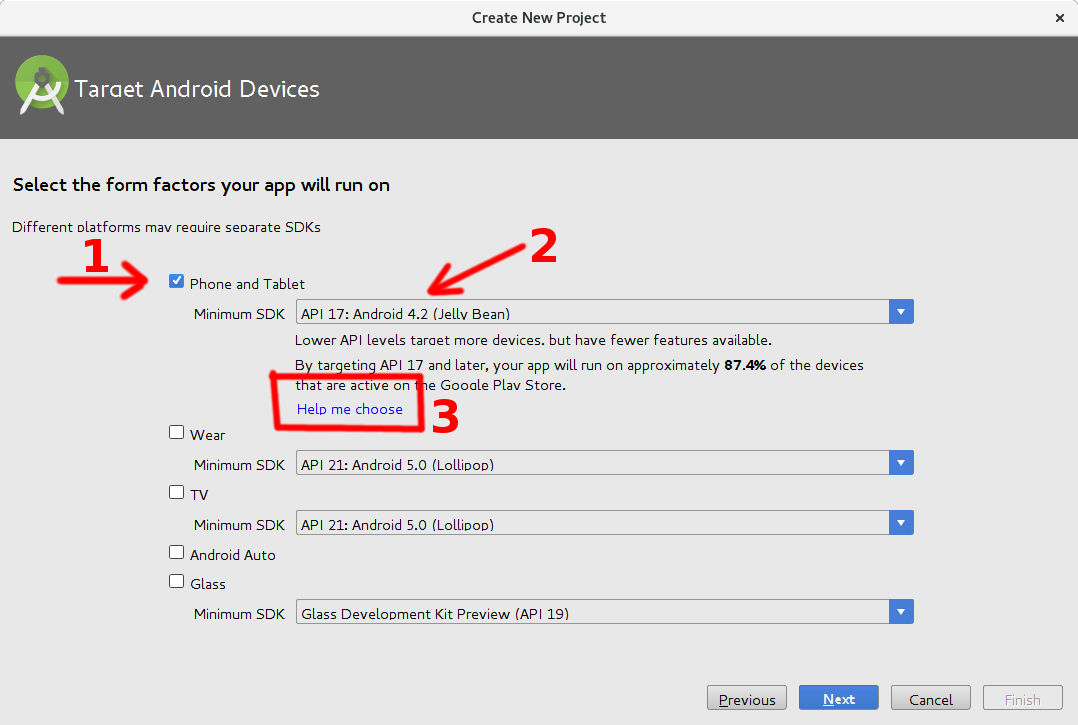
\includegraphics[scale=0.2]{chapters/ch02/images/3_os_select}
\end{center}

\begin{enumerate}
	\item In this course we will be developing only for phones and tables. Check this option and ignore the others.
	\item \textit{Minimum SDK:} This is the minimum version of android API that your app will run on. For example if you selected API 21 (Lolipop) as minimum API then your app will not run on any mobile device that has android version 19 (Kitkat) or less installed on it. For now select API 17 so that our app runs on approximately 87.4\% of the devices out there. 
	\item If you want to see the complete compatibility chart, click ``Help me choose''. This will show you approximate number of devices your app will run on.
\end{enumerate}

Hit next button to go to the ``Add an Activity to Mobile'' screen:

\begin{center}
	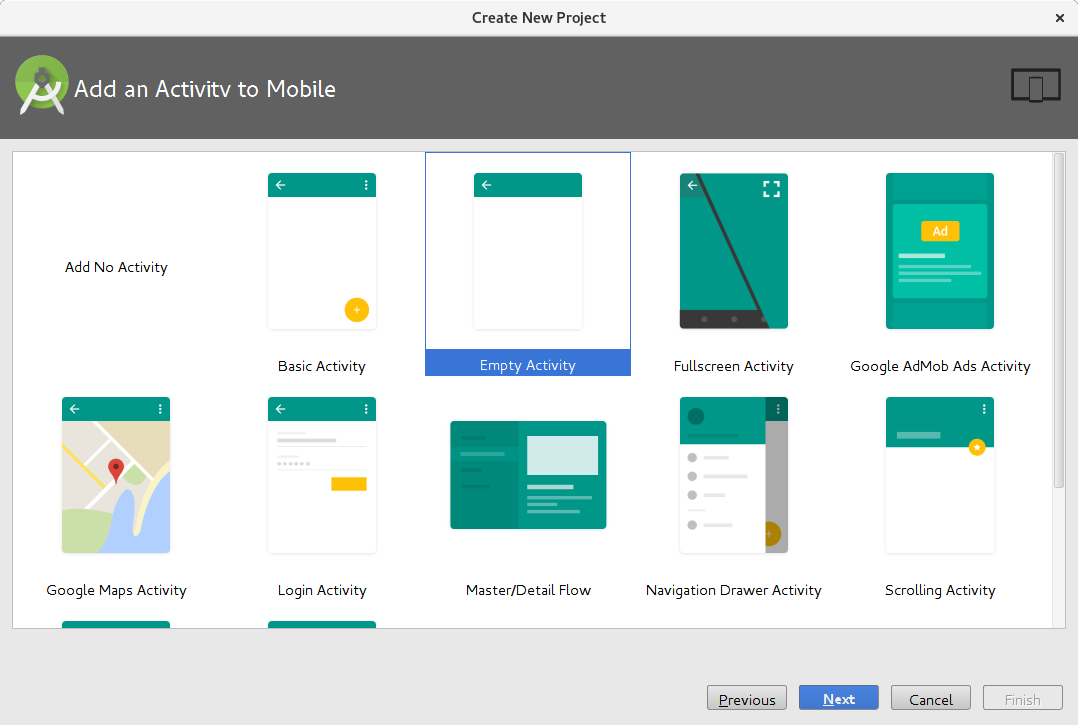
\includegraphics[scale=0.2]{chapters/ch02/images/4_activity}
\end{center}

Select ``Empty Activity'' and hit next to go to ``Customize the Activity'' screen. Leave the default options as is and click finish to create the project.

\section{Tour of Android Studio IDE}
Once your project is successfully created, you will see the following screen with some files already opened up:

\begin{center}
	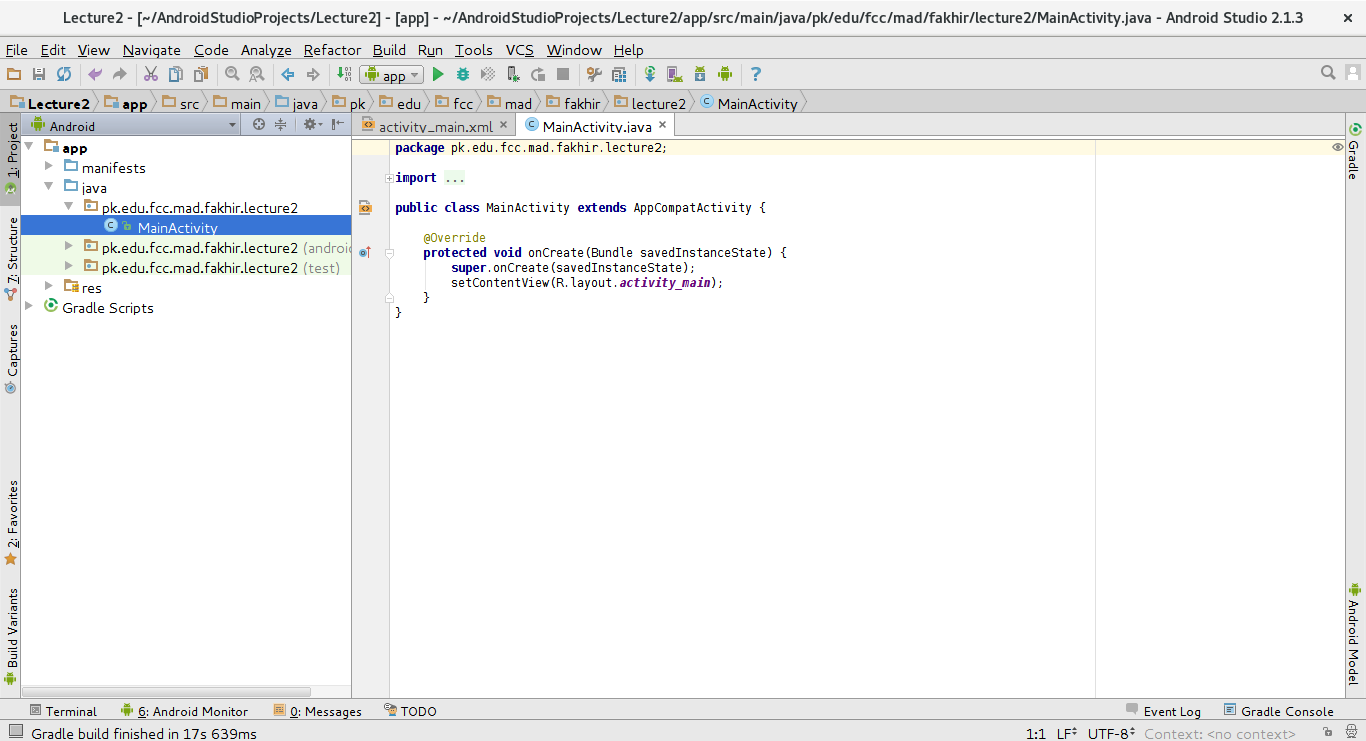
\includegraphics[scale=0.2]{chapters/ch02/images/5_android_studio}
\end{center}

The left side panel shows the project structure. This panel basically shows the assets, code, configuration files related to this project:

\begin{center}
	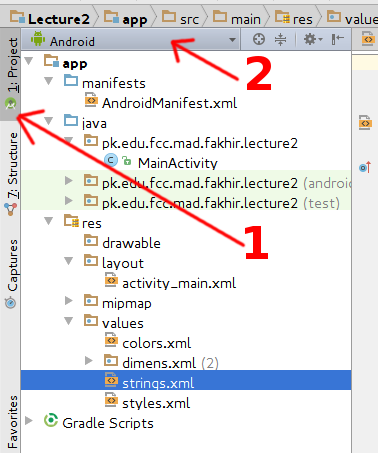
\includegraphics[scale=0.3]{chapters/ch02/images/6_project_panel}
\end{center}

\begin{enumerate}
	\item Make sure that the ``Project'' tab is selected. This will show the overall bird's eye view of the current project. You can view the project structure in various ways as mentioned below.
	\item Now if ``Android'' is selected, this will show you the ``Logical'' layout. Android studio will group and show similar items under the same label even if these items are actually placed in different directories.
	\item If you select ``Project'' instead of ``Android'', this will show you the actual physical structure of the project including all the actual sub-directories. Both the views are useful but for now we will be using ``Project $\rightarrow$ Android''.
	\item ``Structure'' tab shows the code structure of the project i.e: Class hierarchies, member functions, member variables etc.
\end{enumerate}

In the middle of the screen this area is the editor panel. Here we write and modify code. Two files are already opened, one java and other XML. We will look into detail what these files exactly do. Click on the ``activity\_main.xml'' tab to bring ot the layout.

\begin{center}
	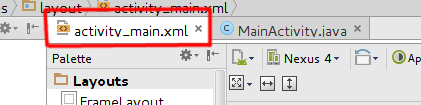
\includegraphics[scale=0.4]{chapters/ch02/images/7_editor}
\end{center}

Clicking any layout XML file opens up the design mode. Notice how the editor area is now converted into a number of panels housing lot of different options:

\begin{center}
	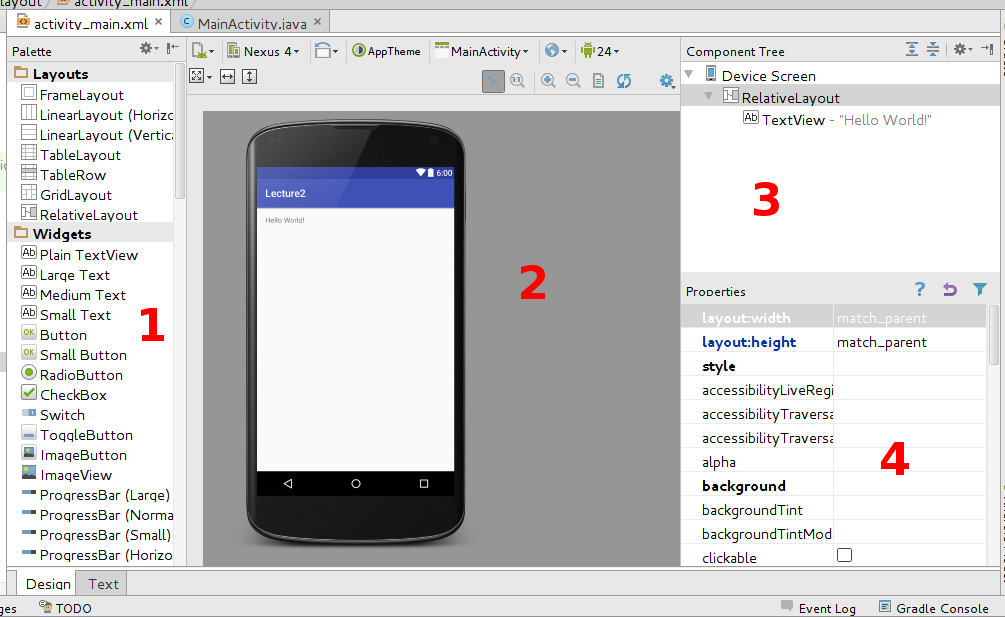
\includegraphics[scale=0.3]{chapters/ch02/images/8_design}
\end{center}

\begin{enumerate}
	\item The panel at the left is referred to as the ``Palette panel''. This panel contains all of the layouts, buttons, widgets, gadgets that you can use to make very complex user interfaces. Just drag anything from here and drop it onto the mobile preview area.
	\item This is the mobile preview area. This shows how your layout will look on the actual device!!! (You don't even have to run your app on the emulator or physical device). 
	
	\textbf{IMPORTANT NOTE: This ONLY previews the layout. This will NOT run your java code. To run your logic code you must run your app on an emulator or a dvice.}
	\item The panel on the top right is called ``Component tree'' panel. This shows hierarchical relationship between different components and controls (for example a button can contain a label inside it etc). 
	\item The panel on lower right shows all of the possible properties of the currently selected component. Here you can change size, color, font, physical outlook etc of any control that you can imagine.
\end{enumerate}

Let's explore the preview area a little bit more. 

\begin{center}
	
\includegraphics[scale=0.6]{chapters/ch02/images/9_design_area}
\end{center}

\begin{enumerate}
	\item You can preview your layout on any android device (phone, tablet, watch or even TV). Clicking on this button will bring down a drop-down menu having a lot of options. You can choose any of the devices to test your layouts onto.
	\item You can test your layout (or user interface in other words) on different orientations. Click this button to switch between portrait and landscape modes.
	\item You can also change the overall theme of your app but for now we will not be covering this.
	\item You can make multiple layouts or screens in your app and you can individually test any of these. Since we have only one layout for our app, the drop-down menu shows only one!
	\item You can also change the language of your app for example from english to arabic.
	\item This zooms and unzooms the preview area.
	\item Refreshes the preview area to update latest changes.
\end{enumerate}

The layouts are actually XML files containing source code. Android studio reads that code and draws the layout in design view. In order to view the actual XML source code, click the ``Text'' tab on bottom left side of the design area, right underneath the ``Palette panel'':

\begin{center}
	
\includegraphics[scale=0.6]{chapters/ch02/images/10_textMode}
\end{center}

This will transform the entire middle area from drag/drop design mode to a source code editor:

\begin{center}
	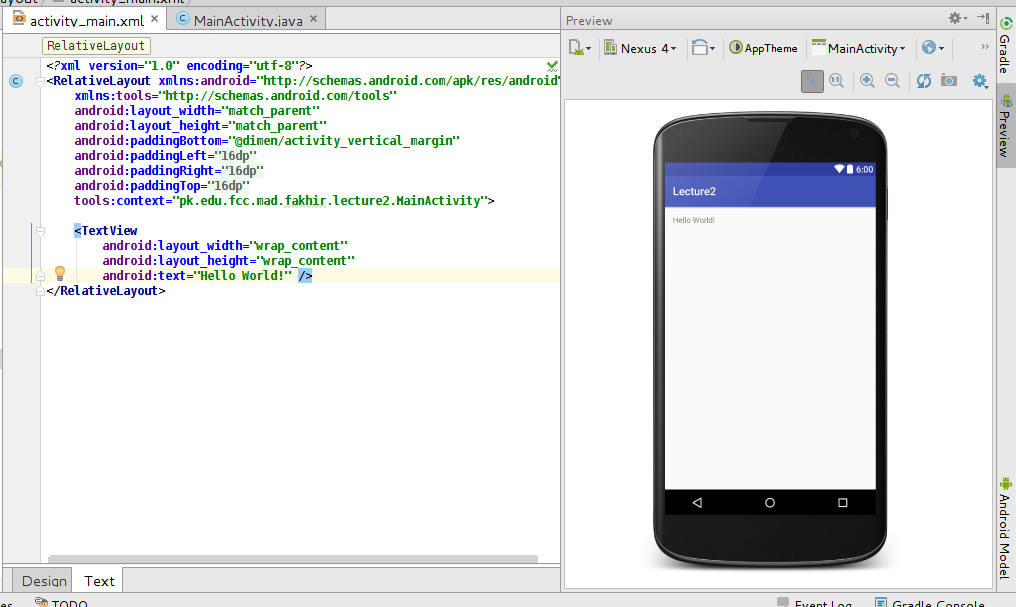
\includegraphics[scale=0.3]{chapters/ch02/images/11_textMode}
\end{center}

On the left side you can see the complete XML source code for the layout. On the right side you can see the preview window. If you like you can make very complex layouts right in this XML text mode!

\section{Important concepts}
Let's pause for a moment and let's take a look at some important concepts.

\subsection{Activity}
\label{TOAS:activity}
An \textbf{Activity} can be thought of as a screen. Like a university website can have multiple pages, about, home, faculty, students etc. Each website has a different ``layout'' or ``appearance''. Similarly a mobile app can have multiple screens or activities.

Each activity is made up of two components: 
\begin{itemize}
	\item Exactly ONE Java file (the brains / logic)
	\item At least ONE XML file (the beauty)
\end{itemize}

\begin{center}
	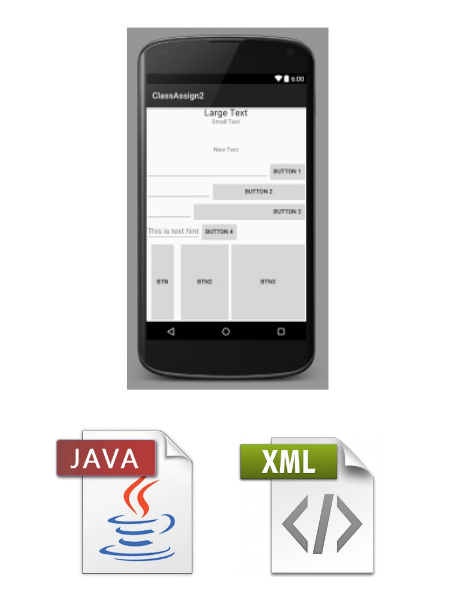
\includegraphics[scale=0.4]{chapters/ch02/images/12_activity}
\end{center}


Our app has got only one activity named \texttt{\textbf{Main}} having ``\texttt{MainActivity.java}'' and ``\texttt{activity\_main.xml}'' attached to it. We can create as many activities as we want within an app, as we will see later down the road.

\subsection{View}
You can think of the views simply as ``(invisible) interactive rectangles''. Pretty much everything is a view. A button is a view, edit box is a view, label is a view etc. There can even be invisible views. Special views that can contain other views within them are called ``View Groups''. Views \textbf{can not} contain any other views. But view groups \textbf{can} contain other views or even view groups. View groups are used to nicely format and align components on the screen.

\section{Simple layout}
Alright, enough theory, let's resume our app development. Open up ``activity\_main.xml'' if it is not already open and go to the design mode. Let's zoom it a bit. Click the zoom button a few times:

\begin{center}
	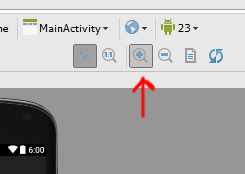
\includegraphics[scale=0.4]{chapters/ch02/images/14_zoom}
\end{center}

You will see \textbf{“Hello world”} written on the output screen. This is actually a UI control of type \texttt{TextView} placed on the screen. \texttt{TextView} displays text to the user and optionally allows them to edit it.

Go to the panel on the right, find the ``Component Tree'' view. The ``Component Tree'' shows all the UI controls, views, view groups placed onto the canvas in a hierarchical parent-child tree like structure. Select \texttt{TextView}. You can either directly select a control from the canvas or the from ``Component Tree'':

\begin{center}
	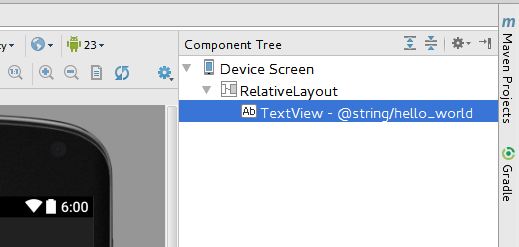
\includegraphics[scale=0.4]{chapters/ch02/images/15_component_tree}
\end{center}

Let's modify some properties of the text view. Under the ``Component Tree'' you will see the properties panel. It lists all of the properties of a selected widget. This panel is ``context sensitive''. It means that the values listed will change depending on the type of widget currently selected. Since we've already selected \texttt{TextView}, find \texttt{textSize} and change it to \textbf{60dp}. The `dp' means device independent points, these are not raw pixels. Also set the \texttt{textStyle} to `Bold' and `Italic':

\begin{center}
	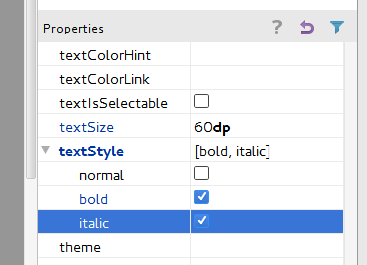
\includegraphics[scale=0.4]{chapters/ch02/images/16_bold_italic}
\end{center}

There are two ways to specify the color. Simplest is the \#RGB. This is means that only 16 levels for each of the red, green and blue colors, a total of only 4096 color combinations. Second way is to specify the entire \#RRGGBB format. This one is 256 levels for each red, green,blue; a total of 16 million color combinations.

While \texttt{TextView} is still selected, enter \#002 in the background field:

\begin{center}
	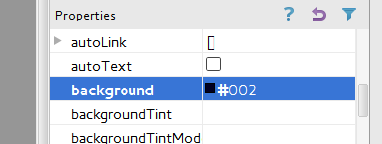
\includegraphics[scale=0.4]{chapters/ch02/images/17_background}
\end{center}

Enter \#ffff33 in \texttt{textColor}:

\begin{center}
	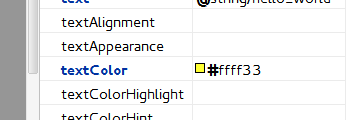
\includegraphics[scale=0.4]{chapters/ch02/images/18_text_color}
\end{center}

Select Nexus 10 tablet to see how our layout looks like on it:

\begin{center}
	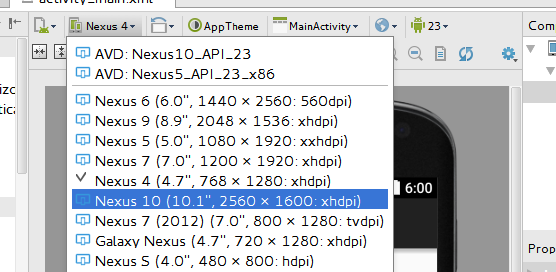
\includegraphics[scale=0.4]{chapters/ch02/images/19_nexus_10}
\end{center}

Now select Nexus 5:

\begin{center}
	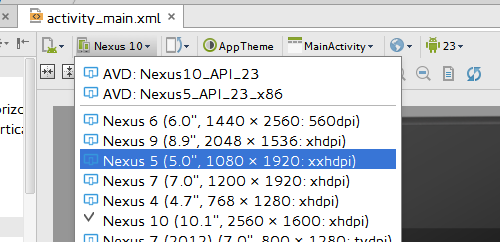
\includegraphics[scale=0.4]{chapters/ch02/images/20_nexus_5}
\end{center}

The mobile phone view may be a bit too zoomed in. Click on `Zoom to fit' button:

\begin{center}
	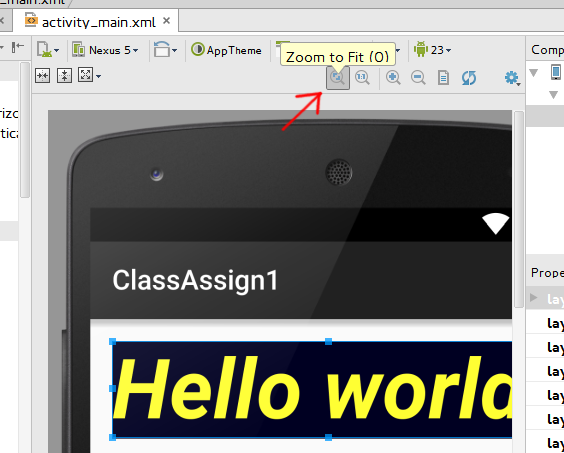
\includegraphics[scale=0.4]{chapters/ch02/images/21_zoom}
\end{center}

To see how your layout looks like on a different orientation such as landscape mode, click the change orientation button:

\begin{center}
	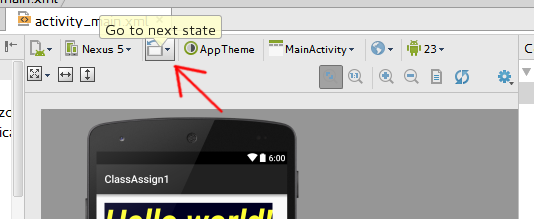
\includegraphics[scale=0.4]{chapters/ch02/images/22_state}
\end{center}

Finally click the green play button to run the app on device or the emulator:

\begin{center}
	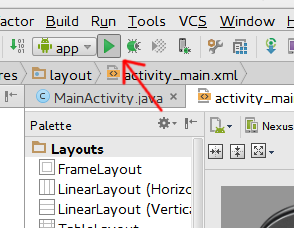
\includegraphics[scale=0.4]{chapters/ch02/images/23_play}
\end{center}

You should see the following on your mobile or the emulator. Quick tip about emulator: To change its orientation from portrait to landscape and vice versa just press `ctrl+F12':

\begin{center}
	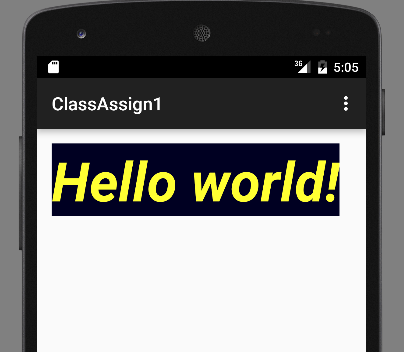
\includegraphics[scale=0.4]{chapters/ch02/images/24_device}
\end{center}

\section{Exercise}
Try to make an interface shown in the following diagram. If you don't understand anything then don't worry we will cover it in detail in the upcoming classes.

\begin{center}
	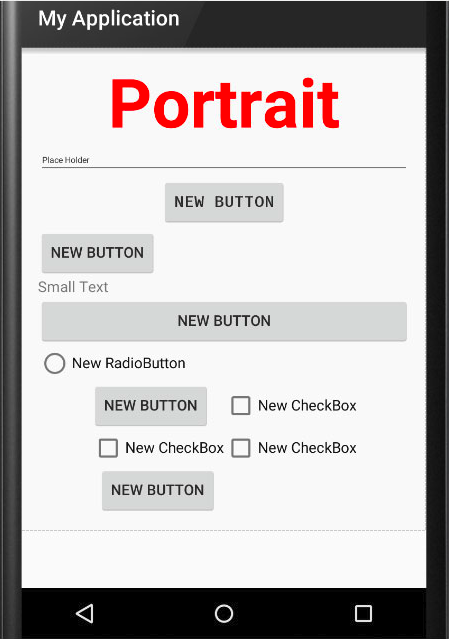
\includegraphics[scale=0.4]{chapters/ch02/images/25_activity1}
\end{center}
\chapter{User Interface Basics}

\section{User interface components}
\subsection{Widget}
What is a widget? Widget is just a fancy name for user interface element or controller for example button, label, check box etc. There are a lot of widgets available in android. In the design mode, if you look at the left side panel called the ``Palette panel'', you would see all of the UI controls or widgets that you can use in your app:

\begin{center}
	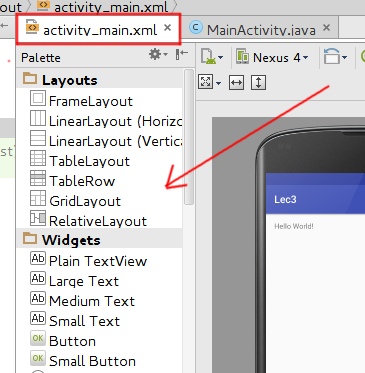
\includegraphics[scale=0.4]{chapters/ch03/images/1_palette_panel}
\end{center}

\subsection{Basic concepts}

\subsubsection{Views}
In android a ``\texttt{View}'' is an interact-able rectangle on the screen. Just like the concept of windows, everything is a window in Windows operating system, pretty much everything is a view in android. So the buttons, text labels, text fields, radio buttons etc all are views. There is actually a class in the android SDK called ``\texttt{View}'' and every widget is inherited from it. For more details on the \texttt{View} class refer to the following link:

\url{https://developer.android.com/reference/android/view/View.html}\\

\underline{\textbf{Very important:}} Unlike windows operating system, a view CAN NOT contain other views in it.

\subsubsection{View groups}
``\texttt{ViewGroup}'' is a \textit{special} type of \texttt{View} (actually it is inherited form the ``\texttt{View}'' class available in android SDK). A view group is a container that can contain other \texttt{Views} or even \texttt{ViewGroups} (these are called ``children''). By building up a hierarchical structure like this you can form very complex user interfaces with ease as shown below:

\begin{center}
	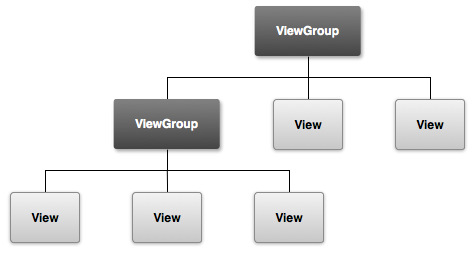
\includegraphics[scale=0.4]{chapters/ch03/images/2_viewGroups}
\end{center}

We have a \texttt{ViewGroup} class in android that is inherited from \texttt{View} class. For more details on the \texttt{ViewGroup} class refer to the following link:

\url{https://developer.android.com/reference/android/view/ViewGroup.html} \\

\underline{Usage:} Some examples of view groups include the \texttt{RelativeLayout}, \texttt{LinearLayout}, \texttt{FrameLayout}, \texttt{GridLayout}, \texttt{Fragments} etc. Generally the view groups are used to contain other widgets and to format or display them nicely on the screen. \\

\underline{\textbf{Very important fact:}} Your app MUST have AT LEAST \underline{ONE} \texttt{ViewGroup} on top (head) of the UI hierarchy. By default when you create a new project the root is set to ``\texttt{RelativeLayout}''.\\

Ok, let's see all of this in action.

\subsection{Widgets and containers in detail}
\subsubsection{Create new project}
\label{sec:createProj}

To complete this class activity let's start fresh and create a new project from scratch. Perform the following steps:
\begin{enumerate}
	\item Create a new project having name ``\texttt{Lec3}''
	\item Select minimum API 16 : Android 4.1 (Jelly Bean).
	\item Select ``\texttt{Empty Activity}''
	\item Accept default values for activity and finish.
\end{enumerate}

\subsubsection{Linear Layout}
Assuming that you've chosen default names, open up the layout file ``\texttt{activity\_main.xml}'' and go to the text mode. Right click on the gray colored gutter on the left side and select ``Show line numbers'':

\begin{center}
	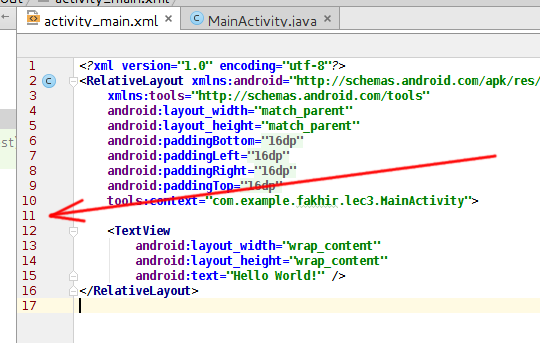
\includegraphics[scale=0.4]{chapters/ch03/images/3_line_numbers}
\end{center}

Go to line 1 and change ``\texttt{RelativeLayout}'' to ``\texttt{LinearLayout}''. Now select and delete lines 6-9. These are the layout attributes or properties. We will look into these in detail later on. Also delete the entire \texttt{TextView} element (lines 8-11). You should have an empty linear layout:

\begin{center}
	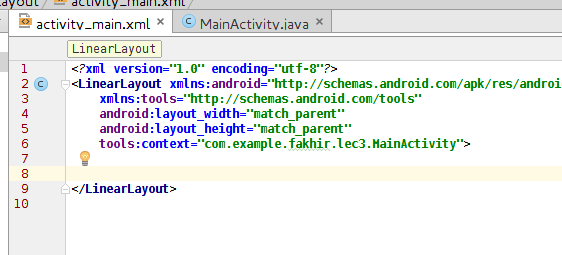
\includegraphics[scale=0.4]{chapters/ch03/images/4_linear_layout}
\end{center} 

\underline{\textbf{\texttt{LinearLayout:}}} A linear layout is a view group. It is inherited from the \texttt{ViewGroup} class. This means that it is a container that can contain buttons, labels etc and even other liner layouts ! A linear layout displays its children in either a horizontal or a vertical arrangement.

Go to th design mode and drag two widgets on top the linear layout as shown below:

\begin{center}
	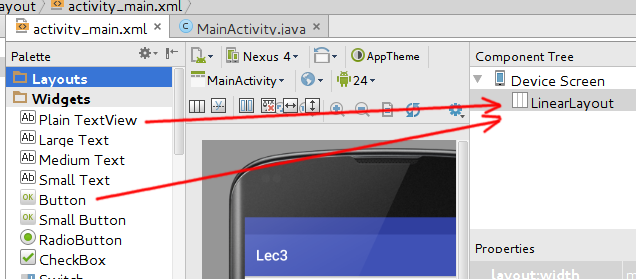
\includegraphics[scale=0.4]{chapters/ch03/images/5_linear_layout}
\end{center} 

Once you've added the widgets to the layout, click to select the ``Linear Layout'' root element from the component tree panel. Change its ``\texttt{orientation}'' property to horizontal. 

Once you've done that, now try changing the orientation to ``vertical'':

\begin{center}
	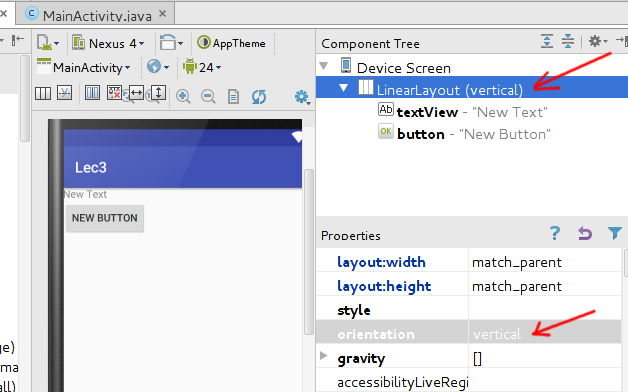
\includegraphics[scale=0.4]{chapters/ch03/images/6_linear_layout}
\end{center} 

Verify that the changes have been correctly updated in the preview panel.\\

Change the label text to ``Hello World !!!'' and button text to ``Click me''. Notice that even though we used mixed case string in both cases but the actual output string on the button is all caps:

\begin{center}
	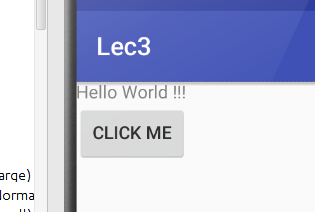
\includegraphics[scale=0.4]{chapters/ch03/images/7_change_text}
\end{center} 

If you want to change this to mixed caps, then switch to text mode. In ``activity\_main.xml'' find the button element. Add an attribute named ``\texttt{android:textAllCaps}'' and set it to \texttt{false}. The preview window will update automatically to reflect the changes:

\begin{center}
	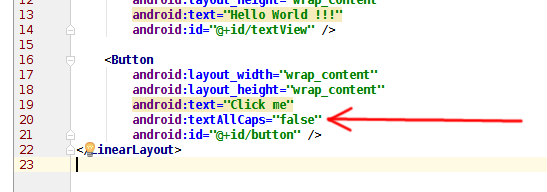
\includegraphics[scale=0.4]{chapters/ch03/images/8_text_case}
\end{center} 

Switch to the design mode and try setting the \texttt{textAllCaps} attribute for our text label to \texttt{true}. \\

You can read more about linear layouts here:

\url{https://developer.android.com/guide/topics/ui/layout/linear.html}

\subsubsection{View dimensions}

While in design mode, from the preview panel in the middle, click on the text label named ``Hello World !!!''. A blue rectangle will appear around it. This blue rectangle shows the current size of that widget. Let's try to change the width of this text view. While text view still selected, on the right side properties panel you should see the ``\texttt{layout:width}'' attribute with a value of ``\texttt{wrap\_content}''. \texttt{wrap\_content} tells the widget to set its width to the smallest size just to contain all of its children. The only child of text view is that text, to the size of the entire controller is adjusted according to that, just like a rubber band wrapped around a bunch of pencils. Thy changing the text to something long and see how the size of the widget changes.

\begin{center}
	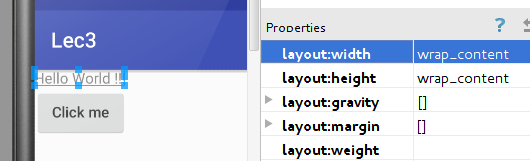
\includegraphics[scale=0.4]{chapters/ch03/images/9_layout_width}
\end{center} 

With text view still selected, change the ``\texttt{layout:width}'' to ``\texttt{match\_parent}''. \texttt{match\_parent} tells the widget to adjust its size to match its parent's size as much as possible (if there are no other widgets in the way). Its like inflating a big-balloon inside a small container. Watch the new size of our text view change to match the boundaries of the phone itself.

\begin{center}
	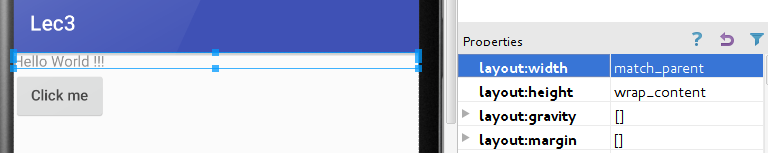
\includegraphics[scale=0.4]{chapters/ch03/images/10_layout_width}
\end{center} 

Try to change the orientation of the device to landscape, you will see that the text view changes its size automatically to match its parent. 

\subsubsection{View Gravity}

Now let's explore some other attributes. Change the ``\texttt{layout:width}'' of the text view back to \texttt{wrap\_content}. Also change the \texttt{background} color to something you like so that we can see its exact size against the white canvas. Find and expand the attribute named ``\texttt{layout:gravity}''. Check the ``right'' field. The text view will snap to the right edge of the screen:

\begin{center}
	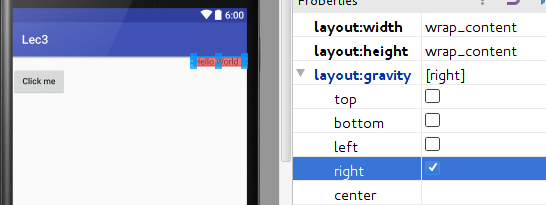
\includegraphics[scale=0.4]{chapters/ch03/images/11_layout_gravity}
\end{center} 

Uncheck ``right'' and click on the ``center'' field, then select ``horizontal'' and see what happens. \\

\underline{\textbf{Note:}} When you are setting \texttt{layout:gravity} the view needs some space to move around or to set its position. If the view doesn't appear to change its position, check the size of its parent. Is the parent big enough to allow the child to move around inside it? \\

After this, now click on the button to select it. Try changing its position through \texttt{layout:width}. Apart from \texttt{layout:gravity} each view also has a separate attribute called \texttt{gravity}. This changes the position of its \textit{``children''}. For example it you set the \texttt{gravity} field of the button to both ``bottom'' and ``center'' the text of the button (which is the child of the button view) will move towards the bottom edge of the button. Optionally also set the \texttt{layout:height} (the height of the button) to 70dp:

\begin{center}
	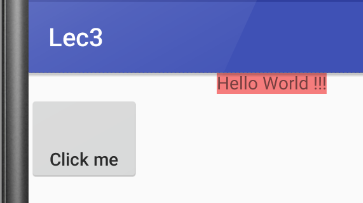
\includegraphics[scale=0.4]{chapters/ch03/images/12_gravity}
\end{center} 

\underline{\textbf{Important distinction:}}\\

\textbf{\texttt{layout:gravity}} $\rightarrow$ Sets the position of the current view inside its parent.

\textbf{\texttt{gravity}} $\rightarrow$ Sets the position of all the children inside the current view (or view group). \\

\subsubsection{Margin and Padding}
As an extra step select the linear layout and change its background to something yellowish. Also change both of its \texttt{layout:width} and \texttt{layout:height} to \texttt{wrap\_content}. \\

\textbf{``Margin'':} It defines how much gap there is between two views (or view groups). If the views don't have any margins around them they will bump into each other. 

\begin{center}
	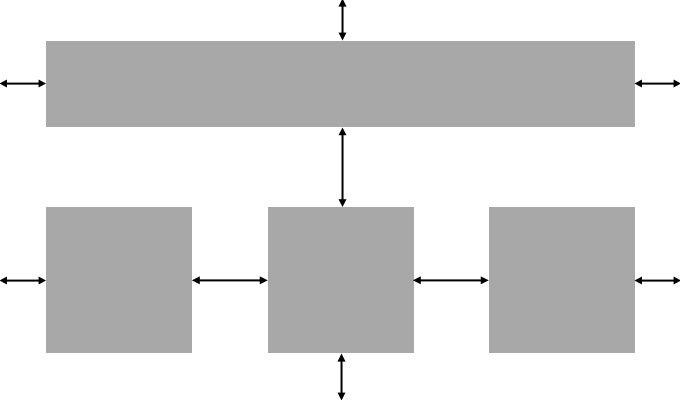
\includegraphics[scale=0.2]{chapters/ch03/images/13_margin_def}
\end{center} 

Select text view again and look for ``\texttt{layout:margin}'' attribute. Change the ``all'' field to \texttt{10dp}. You will notice that there is now a gap of 10 points all around the text label. You can also set the margin individually for each of the view sides. 

\begin{center}
	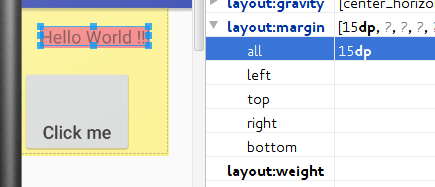
\includegraphics[scale=0.4]{chapters/ch03/images/14_margin}
\end{center} 

\textbf{``Padding'':} This increases te size of the control. Imagine wrapping a box with a very thick foam. 

\begin{center}
	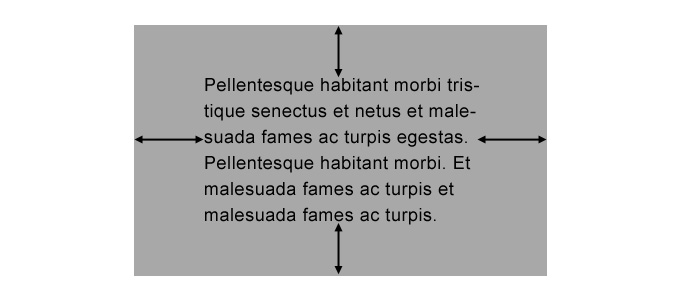
\includegraphics[scale=0.2]{chapters/ch03/images/15_padding_def}
\end{center}

Select text view again and look for ``\texttt{padding}'' attribute. Change the ``all'' field to \texttt{10dp}. You will notice that text view got a bit bigger:

\begin{center}
	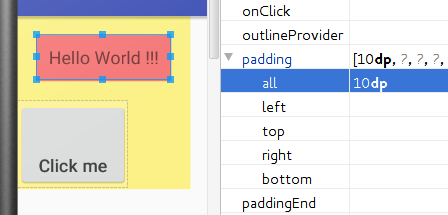
\includegraphics[scale=0.4]{chapters/ch03/images/16_padding}
\end{center}

You can do this with any view or control to customize its outlook.

\underline{\textbf{To summerize:}}

\textit{\textbf{Margin:}} Between border and its parent layout

\textit{\textbf{Padding:}} Between content and border

\begin{center}
	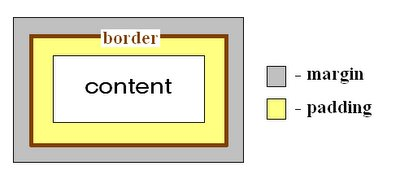
\includegraphics[scale=0.3]{chapters/ch03/images/17_mar_pad}
\end{center}

\subsubsection{Modifying the XML}
Sometimes our required attributes are not present in the design view. To see this, switch to design mode and select linear layout. From the properties panel try to find attributes named ``\texttt{layout:gravity}''. You won't be able to find it. 

Now time to edit some XML, switch to the text mode. Add an attribute named \texttt{layout:gravity} in the \texttt{LinearLayout} element and set it to ``center'':

\begin{center}
	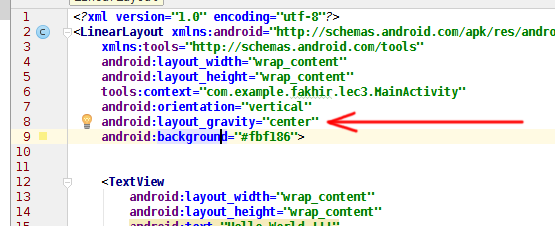
\includegraphics[scale=0.4]{chapters/ch03/images/18_ll_grav}
\end{center}

Once you've done that, the preview window will automatically update to reflect changes:

\begin{center}
	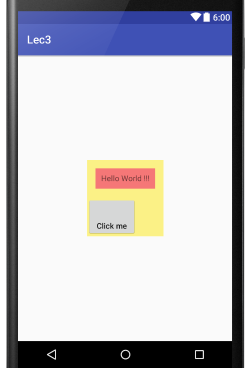
\includegraphics[scale=0.3]{chapters/ch03/images/19_output}
\end{center}

\textit{Tip:} You can exclusively use text mode without ever having to go to the design mode.

\subsection{A bit complex example}
Follow the steps in \hyperref[sec:createProj]{section 1.3.1} create a new project. You can name it something like ``Lec3b'' or ``ClassAssign2'' etc. \\

Go to the text mode, change the layout to linear. Also delete the text view. Make sure that the root layout is empty. Now switch to design mode. Select the \texttt{LinearLayout} from component tree and set its \texttt{orientation} to ``vertical''. Also make sure
that the gravity is unset:

\begin{center}
	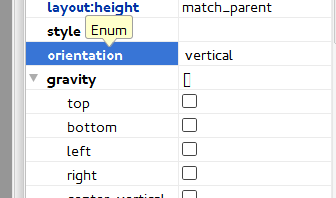
\includegraphics[scale=0.4]{chapters/ch03/images/20}
\end{center}

Now drag a new \texttt{LinearLayout} (horizontal) from the control palette on the left and drop it on top of the parent \texttt{LinearLayout} inside component tree:

\begin{center}
	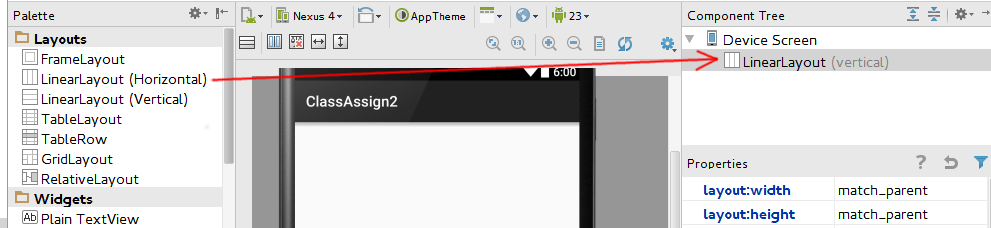
\includegraphics[scale=0.4]{chapters/ch03/images/21}
\end{center}

Select the child linear layout and set its \texttt{layout:height} to ``\texttt{wrap\_content}'':

\begin{center}
	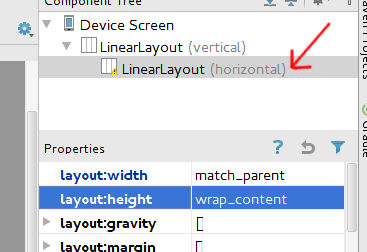
\includegraphics[scale=0.4]{chapters/ch03/images/22}
\end{center}

Drag ``Large Text'' view on top of the child \texttt{LinearLayout}. Set its text to ``Hello !!! This is a test label.'':

\begin{center}
	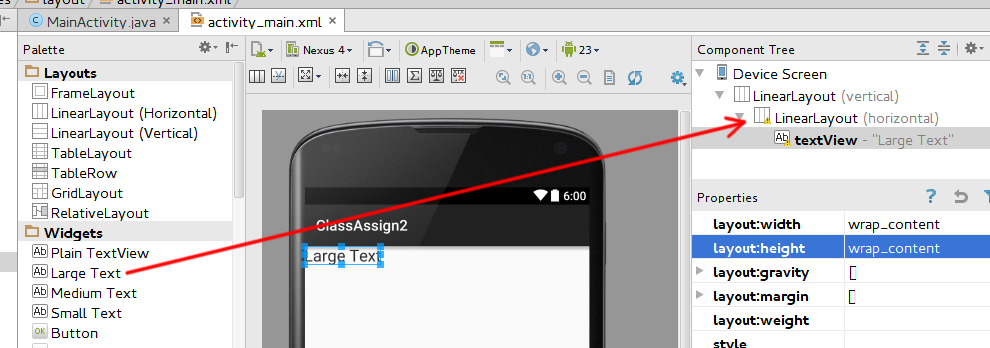
\includegraphics[scale=0.4]{chapters/ch03/images/23}
\end{center}

Drag an \texttt{imageView} on top of child \texttt{LinearLayout}. Change its \texttt{src} parameter to \texttt{@mipmap/ic\_launcher}:

\begin{center}
	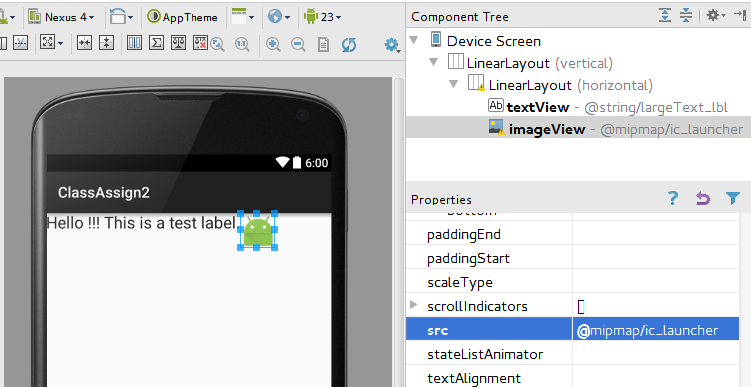
\includegraphics[scale=0.4]{chapters/ch03/images/24}
\end{center}

Go to the text mode and make sure that the preview window is visible. In the xml file, as soon as you place your keyboard cursor on the \texttt{LinearLayout} tag, the layout will be highlighted in the right preview window:

\begin{center}
	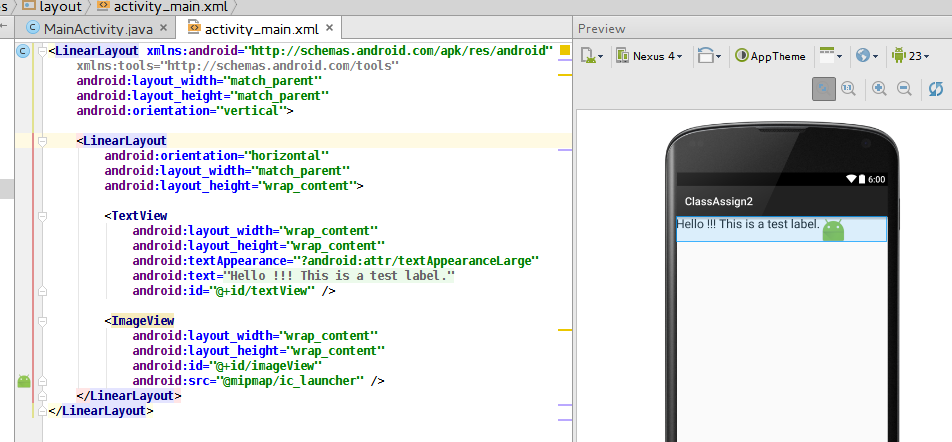
\includegraphics[scale=0.4]{chapters/ch03/images/25}
\end{center}

Remember the gravity parameter arranges the contents inside a view? Go back to the design mode, select the child linear layout and set its \texttt{gravity} to ``\texttt{center\_horizontal}'':

\begin{center}
	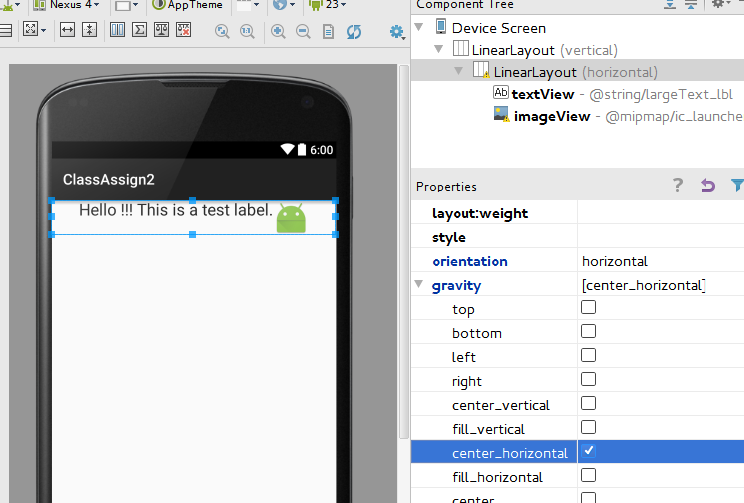
\includegraphics[scale=0.4]{chapters/ch03/images/26}
\end{center}

As we saw earlier that \texttt{layout:gravity} decides how a view is positioned inside a parent. We want the green android image to be right justified. Click on the image view and set its \texttt{layout:gravity} to right. \\

Hmmm, nothing appears to happen !!!

\subsection{Simple Task}
Continuing from the example above:

\begin{enumerate}
	\item Go to the design view. Wrap the image view inside a \texttt{LinearLayout} (vertical). Now try adjusting
	the \texttt{layout:gravity} of the \texttt{imageView} and see if it adjusts itself!
	\item Alternatively you can set the gravity of the \texttt{LinearLayout} to ``right'' yielding the same result. Two
	different ways to do the same thing!
\end{enumerate}

\section{Exercises}
\subsection{Layout 1:}
Produce an output similar to the following:
\begin{center}
	\includegraphics[scale=0.4]{chapters/ch03/images/27}
\end{center}

\subsection{Layout 2:}
Produce an output similar to the following. You can achieve this by combining various orientations of linear layouts:

\begin{center}
	\includegraphics[scale=0.4]{chapters/ch03/images/28}
\end{center}

\textit{\textbf{Warning:}} Hint on the next page.

\newpage
\subsection{Hint:}
Combination of linear layouts. First try to draw view hierarchy tree on a piece of paper. You are completely free to exclusively use \texttt{RelativeLayout} as well!

\begin{center}
	\includegraphics[scale=0.45]{chapters/ch03/images/29}
\end{center}

\section{Homework}
Investigate about the view attribute named ``\texttt{weight}'' and do some practice with it. You can read about it from here:

\begin{enumerate}
	\item \url{https://developer.android.com/guide/topics/ui/layout/linear.html#Weight}
	
	\item \url{http://android.amberfog.com/?p=328}
	
	\item \url{http://www.101apps.co.za/index.php/articles/using-android-s-layout-weight-attribute.html}
\end{enumerate}
\chapter{Resources and Interactivity}

\section{Introduction}
...To be filled...

\section{Android Resources}
A decent android application typically contains many different kinds of assets. It can display images on the screen, play videos, render text, play animations and sounds etc. Assets are an integral part of any mobile app. Usually the artists generate assets and programmers write source code for logic and to present these assets to the user in an effective manner.

In android development assets are referred to as ``Resources''. Almost everything is a ``resource''. A layout is a resource, string table is a resource, an image is a resource. You can include custom resources in your project even if the type and format is unknown to android studio. More information about resources can be found at:

\url{https://developer.android.com/guide/topics/resources/overview.html}

Android studio places all the resources related to each project inside a very special directory called ``\texttt{res}''. Similarly it places all of the source code in a directory called ``\texttt{java}''. Let's explore different types of resources.

\subsection{Create new project}
\label{RAI:createProj}

Create a new project from scratch. Perform the following steps:
\begin{enumerate}
	\item Create a new project having name ``\texttt{Lec4}''
	\item Select minimum API 16 : Android 4.1 (Jelly Bean).
	\item Select ``\texttt{Empty Activity}''
	\item Accept default values for activity and click finish. \\
\end{enumerate}

Once the project is created, go to the panel on the left side, also called the ``project panel''. Make sure that the ``Project'' view is selected from the drop down menu at the top. This view shows the actual physical directory structure of the project as it exists on the hard disk. You can expand any directory by clicking on the little arrow icon present at its left side. \\

All of the project source code and resources are located inside the \texttt{main} folder:

\texttt{Lec4} $\rightarrow$ \texttt{app} $\rightarrow$ \texttt{src} $\rightarrow$ \underline{\textbf{\texttt{main}}}

\begin{center}
	\includegraphics[scale=0.4]{chapters/ch04/images/1_project_panel}
\end{center}

The \texttt{main} folder contains two sub-folders and a very important xml file called ``AndroidManifest.xml'' (this file contains very important app related settings and configurations. We will talk about in detail in future). 

The \texttt{$\backslash$java} folder contains all of the project related source code. The directory structure is similar to the standard java package convention. Try exploring it and see what kind of code is inside it.

The \texttt{$\backslash$res} folder contains all of the project related resources. Sound files, music, images, movies, layout xml, or any custom asset will go into this directory. \\

Let's explore the \texttt{$\backslash$res} a little bit more and see what's inside it. Click and expand \texttt{res}. 

\begin{center}
	\includegraphics[scale=0.4]{chapters/ch04/images/2_res_folder}
\end{center}

As you can see this folder contains a lot of other sub-folders. Each different sub-folder contains different types of resources. For example \texttt{layout} sub-folder contains the layouts for the app, \texttt{drawables} contains pictures and so on. Some sub-folders may have very similar names only differing in the suffix, such as \texttt{mipmap-mdpi}, \texttt{mipmap-hdpi}, \texttt{mipmap-xdpi} etc. These usually contain same types of resources. We will look into it in detail later on. \\

For the time being the two folders we are interested in are the \texttt{layout} and \texttt{values}. As already mentioned ``\texttt{layout}'' contains layout xml files that describes the physical appearance of the activities. ``\texttt{values}'' contains a set of strings (and other types of measurements) that your app will use. \\

For more information on other types of resources please visit \href{https://developer.android.com/guide/topics/resources/available-resources.html}{here}.

\subsection{The String Resource}
Strings are used almost everywhere: on buttons, in labels, alongside radio buttons. There are essentially two categories of strings: 

\begin{enumerate}
	\item The ones used in source code. These are generally for internal system usage, the user can't see these.
	\item The ones that are actually displayed on the app screen. The user will see and interact with these types of strings.
\end{enumerate}

Let's see a practical example. Go to the project panel again. Make sure that ``Project'' mode is selected so that you can view actual physical directory structure. Inside the \texttt{values} folder you should see ``\texttt{strings.xml}'' file:

\begin{center}
	\includegraphics[scale=0.4]{chapters/ch04/images/3_strings}
\end{center}

Double click \texttt{strings.xml}, android studio will open it in the editor. This is a standard xml file format which contains strings to be used in our app (specially the layouts). All of the strings are defined inside \texttt{<resources>} tags:

\begin{center}
	\includegraphics[scale=0.4]{chapters/ch04/images/4_strings_xml}
\end{center}

The actual strings are defined by the \texttt{<string>} tag. Right now there is only one string defined in our app, hence you see only one \texttt{<string>} tag. The name of the string is its ``\textbf{\texttt{id}}'' that you will refer to in your project java code or xml. The text in-between the string opening and closing tags is the actual string that you see on the screen (in this case ``Lec4'').

There are many ways to create new strings: manually, through translation editor or through layout text mode. You can use anyone you like.

\subsubsection{Creating strings manually}
Open up \texttt{strings.xml} in the editor window. Add a new string tag, give it a name ``\texttt{hello\_str}'' and text ``\texttt{Hello World !!!}'' (as done in line 3 below):

\begin{center}
	\includegraphics[scale=0.4]{chapters/ch04/images/5_new_string1}
\end{center}

\subsubsection{Creating strings through translation editor}
Open up any layout file, \texttt{activity\_main.xml} in our case. Go to the design mode, find an ``earth'' icon in the toolbar located at the top of the preview panel, select ``Edit Translations''.

\begin{center}
	\includegraphics[scale=0.4]{chapters/ch04/images/9}
\end{center}

This will open up the translation editor. You can see the string that we created in the previous step. 

\begin{center}
	\includegraphics[scale=0.4]{chapters/ch04/images/11}
\end{center}

Click on the ``+'' button located at the upper left side of the editor. This will open up a small dialog box:

\begin{center}
	\includegraphics[scale=0.4]{chapters/ch04/images/10}
\end{center}

Enter ``\texttt{editor\_str}'' as the key (without quotes) and ``\texttt{This string was created from translation editor}'' as default value (again without quotes). Hit OK. The translator will update to show changes. If you open up \texttt{strings.xml} you will see the new string that we created from translation editor. \\

\textit{So basically the translation editor is just a front end interface for editing \texttt{strings.xml} !!!}

\subsubsection{Creating strings through layout text mode}
Open up ``\texttt{activity\_main.xml}'' and go to line 15. You can see the text of the view is hardcoded as ``Hello World!''. Bring your keyboard cursor onto the ``Hello World!'' string. A small yellow bulb icon will appear to its left side:

\begin{center}
	\includegraphics[scale=0.4]{chapters/ch04/images/12}
\end{center}

Using your mouse cursor click the bulb, this will bring a menu. Select ``Extract string resource'':

\begin{center}
	\includegraphics[scale=0.4]{chapters/ch04/images/13}
\end{center}

This will bring up a dialog box. Enter ``\texttt{new\_Lbl}'' as the ``Resource name''. Remember that string ``name'' is the id of that string resource:

\begin{center}
	\includegraphics[scale=0.4]{chapters/ch04/images/14}
\end{center}

Accept all other values as default and press OK to dismiss the dialog. If you go to the ``\texttt{activity\_main.xml}'' file in text mode, notice that line 15 has now changed. The hardcoded string is replaced with the string resource id:

\begin{center}
	\includegraphics[scale=0.4]{chapters/ch04/images/15}
\end{center}

If you open up ``\texttt{strings.xml}'' you will see a new string created having name as \texttt{new\_Lbl}. \\

Ok go back to ``\texttt{activity\_main.xml}'' and set the text of the view back to the hardcoded ``\texttt{Hello World!}'' so that we can perform the next step!


\subsubsection{Using a string resource}

If not already then open up ``\texttt{activity\_main.xml}'' in text mode to view its xml source. The root layout (which happens to be \texttt{RelativeLayout}) has only one child: a text view (lines 12 to 15). Line 15 is hardcoding the string ``\texttt{Hello World!}'' as the text of the view.

\begin{center}
	\includegraphics[scale=0.4]{chapters/ch04/images/6_new_string2}
\end{center}

Let's replace this hardcoded string with a string resource. Delete the string in line 15 and replace it with ``\texttt{@string/hello\_str}'' (including quotes):

\begin{center}
	\includegraphics[scale=0.4]{chapters/ch04/images/7_new_string3}
\end{center}

The ``\texttt{@string/}'' part means that you are trying to access the string resource. (You can access any type of resource in the text mode by prefixing it with \texttt{@} symbol and then type of the recourse.) The second part is the \texttt{id} or \texttt{name} of the string that you want to use i.e: ``\texttt{hello\_str}''. We created this string earlier, now we are referring to that string resource in our layout file. As you are typing the android studio will show the list of all available strings in the resource file that you can choose from. \\

Switch to the design mode. You will still be seeing ``\texttt{Hello World!!!}'' message in the preview panel, but it is \textbf{not} hardcoded anymore, it is coming from the string resource. If you select the text view and under its properties, check the text attribute. It should show you \texttt{@string/hello\_str} (without the quotes). So instead of text mode, you can also specify string resources through design mode:

\begin{center}
	\includegraphics[scale=0.4]{chapters/ch04/images/8}
\end{center}

\texttt{\underline{Quick Exercise:}} Try changing the text of the text view to our new string resource with name \texttt{new\_Lbl}. Verify that it updates the app outlook properly. \\

\textbf{\underline{NEVER EVER} hardcode a string in your layouts that the user can potentially see}. The reason is that when using string ids in the xml code, if you want to change the language of your app then you just need to replace the \texttt{strings.xml} file with a different \texttt{strings.xml} containing different language strings (same name ids but different text). Your source code will remain EXACTLY the same and you won't have to change even a single line of code !!! \\

\textbf{\underline{WARNING:}} If you ever hardcode strings in your layouts, I'll haunt you in your dreams !!! \\

You can find detailed information about the string resource \href{https://developer.android.com/guide/topics/resources/string-resource.html}{here}.

\subsection{Supporting Multiple Languages}
The general concept is pretty simple. Our app will use string resource ids in the code. Whenever the app needs to display another language, it will \underline{automatically} switch the ``\texttt{strings.xml}'' with another appropriate one!

How does it actually do that? Well if the current language is ``English'', it will load the \texttt{strings.xml} from \texttt{values} directory. But if user selects say french from the phone settings then android OS will automatically load the \texttt{strings.xml} from \texttt{values-fr} directory. Note the suffix ``\texttt{-fr}'', it means french. \texttt{values-ur} is for urdu, \texttt{values-ar} is for arabic and so on. Each of these directories contains \texttt{strings.xml} files having strings of exactly same ids but different texts.

Let's add another language support. Open up the ``translation editor'' and click on the world icon located in the upper left corner of the editor. A huge list of available languages will appear in the drop down list. Select ``French (fr)'':

\begin{center}
	\includegraphics[scale=0.4]{chapters/ch04/images/16}
\end{center}

The translation editor will update itself to include french language. You can now add the french alternatives of the default text \textit{(and yes you need to go to \href{https://www.google.com/search?q=google+translate&ie=utf-8&oe=utf-8}{google translate} and add the translations here manually. Android studio won't magically translate stuff for you!)}. Also add urdu language:

\begin{center}
	\includegraphics[scale=0.4]{chapters/ch04/images/17}
\end{center}

If you go to the project panel at the left side and analyze project directory structure, you'll notice that two new folders have been created to accommodate the new languages i.e: \texttt{values-fr} and \texttt{values-ur}. Each of these folders inturn contain \texttt{strings.xml}. Open these up and see what's inside:

\begin{center}
	\includegraphics[scale=0.4]{chapters/ch04/images/18}
\end{center}

Make sure that the id of the text view is set to \texttt{@string/hello\_str}. Open up \texttt{activity\_main.xml} in design mode. Click on the earth icon located at the upper edge of the preview window, and select any of the available languages that we just added in the previous steps:

\begin{center}
	\includegraphics[scale=0.4]{chapters/ch04/images/19}
\end{center}

The preview should update to reflect new languages:

\begin{center}
	\includegraphics[scale=0.4]{chapters/ch04/images/20}
\end{center}

Also run the app on an emulator or actual phone. Go to your phone settings $\rightarrow$ Language and input $\rightarrow$ Language $\rightarrow$ Francais(France). Now run your app again and you should see following output:

\begin{center}
	\includegraphics[scale=0.4]{chapters/ch04/images/21}
\end{center}

\vskip 3mm
You can visit \href{https://developer.android.com/training/basics/supporting-devices/languages.html}{this} link for more information on supporting multiple languages.

\subsection{Supporting Multiple Orientations}

Suppose that you made an app and it is looking great when in portrait mode. All of buttons and labels appear exactly where you want them to:

\begin{center}
	\includegraphics[scale=0.4]{chapters/ch04/images/22}
\end{center}

Now you switch your phone's orientation to landscape, if you have not designed your layout carefully then it will possibly stretch to account for the new screen size (eg: the \texttt{match\_parent} attribute was set). This stretching can potentially destroy all the aesthetics of your app and make it look hideous:

\begin{center}
	\includegraphics[scale=0.4]{chapters/ch04/images/23}
\end{center}

But if you were careful enough to design your layout so that they do not stretch with the new screen size, then you've got another problem. All of your controls will move to one side of the screen exposing ugly empty space where you could've put extra content:

\begin{center}
	\includegraphics[scale=0.4]{chapters/ch04/images/24}
\end{center}

There is a solution to this problem! Just like when switching to a different language android studio automatically selects the appropriate \texttt{strings.xml} from multiple ones. When switching phone orientations android studio will \textbf{automatically} load the appropriate layout file from multiple ones. \\

\textit{``This means that we need to create multiple layout files having exact same name but possibly completely different content.''} \\

Open up \texttt{activity\_main.xml} in the design mode. Click on the ``Configuration to render this layout'' button located at the top left corner of the preview panel. Then select ``Landscape version'':

\begin{center}
	\includegraphics[scale=0.4]{chapters/ch04/images/25}
\end{center}

This will create a new folder called \texttt{``layout-land''} with a new file named {``activity\_main.xml'}' inside it. You can verify this from the project panel on the left side. When ever the phone is in landscape mode the app will automatically load this layout:

\begin{center}
	\includegraphics[scale=0.4]{chapters/ch04/images/26}
\end{center}

Now with your \texttt{activity\_main.xml} opened, make sure the orientation is switched to the landscape in the design mode. This will automatically load the correct layout xml file. Try to make a layout as shown below:

\begin{center}
	\includegraphics[scale=0.4]{chapters/ch04/images/27}
\end{center}

Now try switching the orientation and see if the correct layout is loaded. Also test this on emulator or the physical device. \\

For more information on supporting multiple orientations please visit: \href{https://developer.android.com/training/multiscreen/screensizes.html}{\textit{Supporting multiple screen sizes}}.

\section{Interactivity}
Before we begin to start coding we need some important concepts, one of which is the resource file.

\subsection{The ``\textbf{\texttt{R}}'' resource file}

Open up \texttt{activity\_main.xml} and go to design mode, make sure it's in portrait mode. Add a button and change it's \texttt{id} to ``\texttt{btn\_click}''. Change the button \textit{text} to ``Click me !!!'' (and you should make a string resource for it):

\begin{center}
	\includegraphics[scale=0.4]{chapters/ch04/images/30}
\end{center}

\textbf{Note:} Text string is completely different from \texttt{id}. The text is what you see displayed on a view. The \texttt{id} is a unique identifier that you will use to refer to the resources and views. Unlike text the \texttt{id} is not visible on the screen, it is used for internal book keeping and referencing resources. \\

Also change the \texttt{id} (NOT the text) of the text view label to ``\texttt{lbl\_hello}''. A dialog box will appear giving a warning to make changes. Click on yes:

\begin{center}
	\includegraphics[scale=0.4]{chapters/ch04/images/31}
\end{center}

\textbf{Tip}: To specify an id just use a string literal, \textit{DO} NOT use a string resource like we used for the text field. \\

Double tap the \texttt{shift} key to open ``Search Everywhere'' dialog. Type ``\texttt{R}''. Two \texttt{R} class files will show up. Double click the one having the same package name as your project. Press \texttt{escape} key to dismiss the search pop-up if it is already there on the screen:

\begin{center}
	\includegraphics[scale=0.4]{chapters/ch04/images/28}
\end{center}

A java file named ``\texttt{R.java}'' will open up in the editor window. This is a very special class automatically generated by android studio. You must NEVER edit it manually (there is even a warning about this shown at the top of the file):

\begin{center}
	\includegraphics[scale=0.4]{chapters/ch04/images/29}
\end{center}

In android every view and every resource has an \texttt{id} assigned to it. The ``\texttt{R.java}'' file contains all the ids of every single thing in your app. There are many inner classes defined inside this file such as \texttt{anim}, \texttt{color}, \texttt{dimen} etc. Each of these contain constant integer member variables. \\

Let's find our button in ``\texttt{R.java}''. Search for ``\texttt{btn\_click}''. Well what do you know! It is just an integer member variable defined in the inner class \texttt{id} and assigned a ``unique'' integer number. We can access this button in the java code as ``\texttt{R.id.btn\_click}'' (line numbers in your case may differ):

\begin{center}
	\includegraphics[scale=0.4]{chapters/ch04/images/32}
\end{center}

Apart from the button, our text view id is also contained inside the \texttt{id} inner class so we can access it as ``\texttt{R.id.lbl\_hello}''. In fact all of the view and view group ids are located under the \texttt{id} inner class.

Do we have string resource ids in here as well? Let's check. Search for any string resource ``name'' that we created earlier such as \texttt{hello\_str}. It is located under the ``\texttt{string}'' inner class. We can access this particular string recourse from our code as ``\texttt{R.}\textbf{\texttt{string}}\texttt{.hello\_str}''. You can also see the ids of other string resources that we created earlier. 

\begin{center}
	\includegraphics[scale=0.4]{chapters/ch04/images/33}
\end{center}

Other resources such as animations, pictures, sounds etc have their ids located under related inner classes.

\vskip 3mm
\textit{To summarize: Whatever id you assign to a view or a resource, it will automatically be converted into an integer member variable inside the ``\texttt{R}'' class and will be assigned a unique integer that you can use later on.}

\subsection{The inflater}
\label{RAI:inflater}
Remember an activity is made up of one or many layouts and exactly one java code file. Let's explore the code in our case. Since our project contains only one activity, there is only one java file. Open up \texttt{MainActivity.java} which is linked to the main activity. 

\begin{center}
	\includegraphics[scale=0.4]{chapters/ch04/images/34}
\end{center}

\texttt{MainActivity} class manages all the logic for this particular activity. Every activity class inherits the \texttt{Activity} class which contains essential code for running an activity. The first thing to notice in the above code is that \texttt{MainActivity} inherits \texttt{AppCompatActivity} class. \texttt{AppCompatActivity} basically extends \texttt{Activity} class to provide necessary support for action bar on older devices. You can find out more information about the \texttt{Activity} class \href{https://developer.android.com/reference/android/app/Activity.html}{here} and info about \texttt{AppCompatActivity} \href{https://developer.android.com/reference/android/support/v7/app/AppCompatActivity.html}{here}. \\

On line 9 there is a method called \texttt{onCreate}. Notice that this is a virtual function and it needs to be overridden (like its done above). When ever your activity is launched \texttt{onCreate} method is the first one to be called. For now ignore its parameters.

Line 10 is calling the \texttt{onCreate} for base class. Normally you don't have to modify this line.

Line 11 The \texttt{setContentView} method is something called an ``\textbf{inflator}''. An inflator basically takes an xml description of a layout and instantiates actual java objects that you see on the screen. Here it is taking \texttt{R.layout.activity\_main} and parses ``\texttt{activity\_main.xml}'' from the ``\texttt{layout}'' folder. When the device orientation is changed the activity is restarted and \texttt{onCreate} method is called. But this time depending on the orientation the inflator will automatically choose \texttt{activity\_main.xml} from ``\texttt{layout-land}'' folder and inflates a layout according to that. 

More information on layout inflators can be found \href{https://developer.android.com/reference/android/view/LayoutInflater.html}{here} and \href{http://stackoverflow.com/questions/2335813/how-to-inflate-one-view-with-a-layout}{here}. \\

Let's quickly create a new layout file. Select the ``Android'' mode from the project panel. Find the ``layout'' group and right click on it:

\begin{center}
	\includegraphics[scale=0.4]{chapters/ch04/images/39}
\end{center}

From the pop-up menu select ``New $\rightarrow$ Layout Resource file''. A dialog box will appear. Enter any name you want, say ``my\_text\_layout''. You can also specify the root element of the layout. When you create a new project the default root is the relative layout. But in this case the default is the linear layout, exactly what we want. For other fields accept the defaults and hit OK:

\begin{center}
	\includegraphics[scale=0.4]{chapters/ch04/images/40}
\end{center}

Now a new layout file named ``\texttt{my\_test\_layout.xml}'' should be created in your project directory. Open it up and create any simple layout that you want, such as following:

\begin{center}
	\includegraphics[scale=0.4]{chapters/ch04/images/41}
\end{center}

We've created a new layout. We can now refer it in our code as ``\texttt{R.layout.my\_test\_layout}''. Go back to \texttt{MainActivity.java} and modify the line 12 as follows:

\begin{center}
	\includegraphics[scale=0.4]{chapters/ch04/images/42}
\end{center}

The \texttt{setContentView} inflator function will parse our new xml and inflate a totally new layout on the screen. Run the app to see the changes on the device:

\begin{center}
	\includegraphics[scale=0.4]{chapters/ch04/images/43}
\end{center}

Great, this tells us that we can use ANY layout file that we want anywhere we want and whenever we want with any activity we want! \\

\underline{\textbf{Important:}} Now undo the changes you've just made and modify line 12 back to the following:

\texttt{setContentView(R.layout.activity\_main);}

because the next sections are relying on that.


\subsection{Output Log}
You can print different log messages to the dedicated console window. This is extremely useful for debugging. Inside the \texttt{onCreate} method add the code shown in line 14 below:

\begin{center}
	\includegraphics[scale=0.4]{chapters/ch04/images/35}
\end{center}

As you start typing the keywords android studio will try to auto-complete and show you a pop-up of multiple options to select from. Choose \texttt{Log.d}. The \texttt{d} stands for debug output. You can use \texttt{Log.e} to print an error. 

\texttt{Log.d} takes two parameters. The first one is something called a TAG. TAG  is used to identify the source of a log message, so we named it ``\texttt{MainActivityTAG}'' here. The second parameter is the actual message that you want to print on the console.

Run the app on emulator or the device. You should see the android monitor panel appeared on the bottom side of the screen. If not then click ``Android Monitor'' tab located at the very bottom edge of the screen:

\begin{center}
	\includegraphics[scale=0.4]{chapters/ch04/images/36}
\end{center}

Make sure that the ``Logcat'' tab is selected. Also make sure that you've selected the correct device and also the correct package related to this particular app:

\begin{center}
	\includegraphics[scale=0.4]{chapters/ch04/images/37}
\end{center}

The android monitor window shows all sorts of messages being dumped on the screen. It is really hard to find our log message that we displayed from all of this huge pile. Go back to the activity monitor and make sure that the ``verbose'' mode is selected and also ``Show only selected application'' is selected from the drop down menu at the right (shown below). Remember the TAG string we gave in \texttt{Log.d}? As you type the TAG in the search field, only the related messages will filter out and you'll see just a handful of messages on the console:

\begin{center}
	\includegraphics[scale=0.4]{chapters/ch04/images/38}
\end{center}

Find out more about the logging \href{https://developer.android.com/reference/android/util/Log.html}{here}. \\

\subsection{Getting View Reference}
You can get the reference to any view via it's \texttt{id}. Remember that after inflating the views become java object at run-time. There is a method called \underline{``\texttt{findViewById}''} which takes the id of a view as argument and returns reference to the view object in memory. 

More information about \texttt{findViewById} is given \href{https://developer.android.com/reference/android/view/View.html}{here}. \\

\subsection{Changing View attributes dynamically}
Let's change the text of our button and the text view label present on out \texttt{activity\_main.xml} layout (portrait mode). Remember that we set the view ids as follows:

\begin{center}
	\includegraphics[scale=0.4]{chapters/ch04/images/44}
\end{center}

Open up \texttt{MainActivity.java} and inside the \texttt{onCreate} method add the following lines:

\begin{center}
	\includegraphics[scale=0.4]{chapters/ch04/images/45}
\end{center}

Also remember that the ids of the views are stored in the \texttt{id} inner class inside the \texttt{R} class. Line 17 is accessing the id of our text label as \texttt{R.id.lbl\_hello} and passing it as argument to the ``\texttt{findViewById}'' method. Then \texttt{findViewById} returns a \texttt{View} object which needs to be casted into \texttt{TextView} type and then finally stored in the reference variable named \texttt{tv}.

Line 18 is then accessing the attributes for this particular and setting it through code. Here we are setting the text of the label. You can set ANY attribute imaginable through this method.

Lines 20 and 21 are getting reference to the button and changing its text. When you run the app you will see the following output:

\begin{center}
	\includegraphics[scale=0.4]{chapters/ch04/images/46}
\end{center}

Alternatively, instead of giving hard-coded string literals you can specify the string resource ids to set the text for any view (line 18):

\begin{center}
	\includegraphics[scale=0.4]{chapters/ch04/images/47}
\end{center}

\subsection{Interacting with the Views}
Bunch of pretty buttons on the screen is no good if they do anything. Whenever a user interacts with a view an event is generated. Whenever an even is generated a special function known an event handler is called (more information about the concept of events and event handlers can be found \href{https://en.wikipedia.org/wiki/Event_(computing)}{here}). 

The event handlers in android must have the following signature:

\begin{verbatim}
public void MethodName(View view) {
    ...
}
\end{verbatim}

It must be a public method having return type \texttt{void}. It must have exactly one parameter of type \texttt{View}. This represents the view object that called this event handler. 

Let's add an event handler for our button using the simplest possible method. We will see other methods in future lectures. \\

Open up \texttt{activity\_main.xml} (portrait mode) and switch to the text mode. Inside the \texttt{<Button>} tag add an \texttt{onClick} attribute and assign it any name such as \texttt{onBtnClickFn} (line number 26 shown below):

\begin{center}
	\includegraphics[scale=0.4]{chapters/ch04/images/48}
\end{center}

Bring the keyboard cursor on the \texttt{onBtnClickFn} string literal. A yellow bulb will appear on the left side. Click it and select ``Create in `onBtnClickFn(View)' MainActivity'':

\begin{center}
	\includegraphics[scale=0.4]{chapters/ch04/images/49}
\end{center}

This will automatically create an event handler method and link it to the button. Go to \texttt{MainActivity.java} and you'll see the method created in the \texttt{MainActivity} class. Whenever you click the button this method will be executed:

\begin{center}
	\includegraphics[scale=0.4]{chapters/ch04/images/50}
\end{center}

\subsection{Controlling views from other views}

Let's change the label text whenever our button is clicked. Open up \texttt{MainActivity.java} and go to our newly created event handler method \texttt{onBtnClickFn}. Add the following lines:

\begin{center}
	\includegraphics[scale=0.4]{chapters/ch04/images/51}
\end{center}

Line 25 gets the reference to the text view object. 

Line 26 sets the desired text whenever the button is clicked. \\

Run the app, click the button and see if the text is changed:

\begin{center}
	\includegraphics[scale=0.4]{chapters/ch04/images/52}
\end{center}

\section{Exercise: Tip calculator}

Create an app that calculates tip to be paid using simple information entered through edit text fields:

\begin{center}
	\includegraphics[scale=0.4]{chapters/ch04/images/53}
\end{center}

\subsection{Solution:}
\underline{\textbf{Warning}}: The next page contains the solution to this exercise. Try it yourself first before viewing the solution.

\newpage
Only the event listener function and logic is shown (you can appropriately set the id's of the views in the layout file yourself):
\begin{center}
	\includegraphics[scale=0.4]{chapters/ch04/images/54}
\end{center}

\chapter{More Interactivity and Dynamic Views}

\section{Introduction}
...To be filled...

\section{More on Event Handlers}
In this section we will explore more about event handlers. We will also see numerous ways to create them and hook them to the widgets.

\subsection{Create New Project}
\label{sec:createProj}

Create a new project from scratch. Perform the following steps:
\begin{enumerate}
	\item Create a new project having name ``\texttt{Lec5}''
	\item Select minimum API 16 : Android 4.1 (Jelly Bean).
	\item Select ``\texttt{Empty Activity}''
	\item Accept default values for activity and click finish. \\
\end{enumerate}

\subsection{Adding Event Handlers outside Java Code}
Modify \texttt{activity\_main.xml} layout so that it has four buttons on it and label them according to the following figure. Also set their \texttt{id's} as shown in the ``component tree'' on the right side. Note that the root element is set to \texttt{LinearLayout}:

\begin{center}
	\includegraphics[scale=0.4]{chapters/ch05/images/1}
\end{center}

Event handlers are callback functions in your code that handle a particular event such as a user click or timer expire etc. There are a few ways to ``attach'' event handlers (also known as ``callback listeners'') to the views. Let's look at various ways to do that:

\subsubsection{Through Layout XML Code}
We've already seen this method in previous lecture (please refer to lecture 4 notes, section 3.6 for more details). To recap, this is one of the easiest methods to attach an event listener to a view. 

Open up \texttt{activity\_main.xml} and switch to the text mode. Find the \texttt{<Button>} tag having text ``\texttt{XML}'' and id ``\texttt{btnXML}''. Add an \texttt{onClick} attribute and name it \texttt{onBtnXMLClicked} (line number 19 shown below):

\begin{center}
	\includegraphics[scale=0.4]{chapters/ch05/images/2}
\end{center}

Bring the keyboard cursor on the \texttt{onBtnXMLClicked} string literal. A yellow bulb will appear on the left side. Click it and select ``Create in `onBtnXMLClicked(View)' MainActivity'':

\begin{center}
	\includegraphics[scale=0.4]{chapters/ch05/images/3}
\end{center}

This will automatically create an event handler method and link it to the button. Go to \texttt{MainActivity.java} and you'll see the method created in the \texttt{MainActivity} class. Whenever you click the button this method will be executed:

\begin{center}
	\includegraphics[scale=0.4]{chapters/ch05/images/4}
\end{center}

Go ahead and add a log message in it, or a \texttt{Toast} if you are feeling adventurous.
You can find more about toasts \href{https://developer.android.com/guide/topics/ui/notifiers/toasts.html}{here}. Run the app on a device or emulator to see if the \texttt{XML} button is working.

\subsubsection{Through Layout Design Mode}
Let's implement the second button labeled ``Design''. Open up \texttt{MainActivity.java} and \textit{manually} add the following function (your line numbers may be different). Notice that the name of the function is greyed out. This is because we haven't hooked it to any view (button in our case) yet:

\begin{center}
	\includegraphics[scale=0.4]{chapters/ch05/images/5}
\end{center}

Event listener functions MUST have exactly the same signature as shown above. Please refer to Lecture 4 notes, section 3.6 for more details about function signatures. \\

Now switch to the design mode. Make sure that you've selected ``Design'' button. Go to the properties panel and in the \texttt{onClick} attribute add the name of the method we are trying to hook i.e: \texttt{onBtnDesignClicked}:

\begin{center}
	\includegraphics[scale=0.4]{chapters/ch05/images/6}
\end{center}

When you run the app you will see the correct message printed on the console when you click the ``Design'' button. For more information about Log messages please refer to Lecture 4 notes section 3.3.

\subsection{Adding Event Handlers from Java Code}
\subsubsection{Anonymous Inner Classes}
\label{sec:anonInnerClass}

\textit{This is a very important section, please read it very carefully and make sure that you've understood everything. Read it multiple times if you have to!} \\

In java the functions are NOT first class. This means that you can't pass functions as parameters or return functions from other functions. You can't even have references to the functions. Unlike C++, there is no concept of a function pointer in Java. This means that you can't do the following:

\begin{verbatim}
public void MyFunction(){
    ...
}

someObj.SomeFunction(MyFunction); // <-- WRONG !!!
OR
someObj.memberVar = MyFunction;   // <-- WRONG !!!
\end{verbatim}

But this means trouble! Then how do we attach event listener functions to the view objects? It appears that there is a way. We can't have references to functions and we can't pass functions as parameters to other functions. But we CAN pass objects as parameters to other functions! So we can exploit this fact and do the following: 

\begin{quote}
	\textit{Instead of trying to pass a function into the parameter, wrap that function inside of an object and then pass that object as a parameter instead.}
\end{quote}

Pseudo-code is given below:

\begin{verbatim}
interface BaseClass{
    public void MyFunction();
}
class MyNewClass implements BaseClass{
    @override public void MyFunction(){
        ...
    }
}
BaseClass myObj = new MyNewClass();
someObj.SomeFunction(myObj); // <-- CORRECT !!!
OR
someObj.memberVar = myObj;   // <-- CORRECT !!!
\end{verbatim}

This is called the ``Command Design pattern''. You can learn more about this design pattern by clicking \href{https://en.wikipedia.org/wiki/Command\_pattern}{here}.\\

There is an interface having a single function in android called ``\texttt{OnClickListener}''. You need to inherit and override this interface and then you can pass that object as parameters which includes the ``\texttt{onClick()}'' method. You can view more details \href{http://developer.android.com/reference/android/view/View.OnClickListener.html}{here}. \\

To summerize, this is what you need to do:
\begin{enumerate}
	\item Extend \texttt{View.OnClickListener} and override \texttt{onClick} method.
	\item Create an object of that child class and pass it as parameter to the view to attach event listener:
	\begin{verbatim}
	class MyNewClass implements OnClickListener{
	@override public void onClick(View view){
	...
	}
	}
	OnClickListener mylistener = new MyNewClass();
	button.setOnClickListener(mylistener); // <-- CORRECT !
	\end{verbatim}
	
\end{enumerate}

\vskip 3mm
But instead of defining a new class (\texttt{MyNewClass} in this case), \textit{java provides special syntax which allows us to declare and instantiate a class at the same time}, called the ``Anonymous Inner Class''. Unlike the regular class syntax, anonymous inner class syntax is an expression. \textit{This is a nameless or throw-away class that you declare right where you want to use it.} For example, above code would become (and is exactly the same as) following:

\begin{verbatim}
OnClickListener mylistener = new OnClickListener{
@override public void onClick(View view){ 
... 
} 
};
button.setOnClickListener(mylistener);
\end{verbatim}

Or alternatively you can even skip the extra variable and create anonymous inner right inside the parameters:

\begin{verbatim}
button.setOnClickListener(new OnClickListener{
@override public void onClick(View view){ 
... 
} 
});
\end{verbatim}

View more on Anonymous Inner Classes \href{https://docs.oracle.com/javase/tutorial/java/javaOO/anonymousclasses.html}{here}.

\subsubsection{Through Java Code: Method 1}
Armed with new knowledge now we are ready to add event listeners to ANY view object. \\

Open up \texttt{MainActivity.java} and go to the \texttt{onCreate} function. Add the code shown in following figure from lines 16 to 23: 

\begin{center}
	\includegraphics[scale=0.4]{chapters/ch05/images/7}
\end{center}

\begin{itemize}
	\item \textit{Line 16:} First we get the reference of button having id ``\texttt{btnCode1}'' and text label ``Code1''.
	\item \textit{Line 17-22:} Here we create a listener object. If you don't understand this then please refer to the ``anonymous inner classes'' section \ref{sec:anonInnerClass} of this document. IMPORTANT: DO NOT forget the semi-colon at the end of line 22 !!!
	\item \textit{Line 23:} Finally we pass the listener object through button's \texttt{setOnClickListener} method. When this button is clicked the listener object's \texttt{onClick} method will be executed.
\end{itemize}

\begin{quote}
	\textit{``TIP: You can use the same listener object on many views. However you would have to detect the view ids inside the \texttt{onCLick} function in order to know which view got clicked''.}
\end{quote}

Let's add event listener to the last button! Go to line 25 and add the following lines of code (lines 25-31). Notice that this time we are declaring the anonymous inner class right inside the function parenthesis (a bit of short-cut to the above code):

\begin{center}
	\includegraphics[scale=0.4]{chapters/ch05/images/8}
\end{center}

Run the app and make sure that all of the buttons are working properly.

\begin{quote}
	\textit{``There are advantages of using anonymous inner classes. You can attach listeners at run-time (as opposed to xml layouts where it must be done at compile time). You can attach as many event listeners to as many views as you like WITHOUT ever defining new member function inside the \texttt{MainActivity} or any other class! This method has its disadvantages though, one is the possibility of code repetition, but that is relatively rare.''}
\end{quote}

\subsubsection{Through Java Code: Method 2}
Now we will see another method to hook event listeners to the views. General idea is to inherit the main activity class from \texttt{View.OnClickListener} interface and then override the \texttt{onClick} virtual function to catch any click events. \\

Inherit the \texttt{MainActivity} class from \texttt{View.OnClickListener} interface. This will turn your main activity class into a big huge listener object which you can pass into the function parameters!!!

\begin{center}
	\includegraphics[scale=0.4]{chapters/ch05/images/9}
\end{center}

The project can't compile yet because we must implement ALL the interface methods! The \texttt{View.OnClickListener} interface contains only a single abstract method \texttt{onCreate} that we must override.You can learn more about the \texttt{View.OnClickListener} interface \href{http://developer.android.com/reference/android/view/View.OnClickListener.html}{here}.\\

Right click anywhere inside \texttt{MainActivity} class and select ``Generate'' or press ``Alt + Insert''. A little menu will pop up. Select ``Override Methods''. Then a dialog box with huge amount of interfaces with all the abstract methods will open up. You may have to collapse some of the items. Roughly near the bottom there will be our desired interface \texttt{android.view.View.OnCLickListener} having an \texttt{onCLick} method underneath it. 

\begin{center}
	\includegraphics[scale=0.4]{chapters/ch05/images/10}
\end{center}

Click on the \texttt{onCLick} method and hit OK. A new method named \texttt{onCLick} will be created inside the \texttt{MainActicity} class by the android studio:

\begin{center}
	\includegraphics[scale=0.4]{chapters/ch05/images/11}
\end{center}

This class can now function as a listener object on its own. We will exploit exactly this fact. Remember that we created new listener objects and passed into the \texttt{setOnClickListener} method? Now we will just pass \texttt{MainActicity} as the listener object.

Go to the onCreate method and delete all the code from previous tasks that we wrote, bringing the method back to its original shape as follows:

\begin{center}
	\includegraphics[scale=0.4]{chapters/ch05/images/12}
\end{center}

Inside \texttt{onCreate} Method, get reference to the buttons and add event listener by passing ``\texttt{this}'' as the listener object! (Specially note lines 17 and 20):

\begin{center}
	\includegraphics[scale=0.4]{chapters/ch05/images/13}
\end{center}

Almost done! Finally go to the \texttt{onClick} method. Since in this section we are passing ``\texttt{this}'' to every view as the listener object. When ever any view is clicked, the \texttt{onClick} method of the \texttt{MainActivity} class will be called: 

\begin{center}
	\includegraphics[scale=0.4]{chapters/ch05/images/14}
\end{center}

Run your app and try clicking the buttons and see what messages you get on the console.

\begin{quote}
	\textbf{Pop Quiz:} Why are we passing ``\texttt{this}'' as a parameter to the set listener method?
\end{quote}

\subsubsection{Exercise}

You have to write code inside the \texttt{onClick} method shown above and properly handle both the Code 1 and 2 buttons. (SPOILER: Solution is given on the next page!)

\newpage

\textbf{Solution:}
\begin{center}
	\includegraphics[scale=0.4]{chapters/ch05/images/15}
\end{center}

\vskip 3mm
You can mix and match any of the methods (1,2,3,4) described above in any combination you like.

\section{Dynamic Views}
Let's start fresh. Create a new project (follow section \ref{sec:createProj}). Name your project as \texttt{Lec5b}.

Any widget or a view or a view group that you can add through XML or the design mode you can add purely through programming. Every single field for every single view that you can change in design mode, you can also change through code. Every widget has a corresponding java class that we can use to instantiate and display the widget on the screen through code. It is entirely possible to create very complex layouts completely inside java code. \\

\subsection{Setting up the Layout file}
From your \texttt{activity\_main.xml} layout file, delete the default \texttt{TextView} and change the layout from Relative to Linear (vertical): \textbf{EXTREMELY IMPORTANT}: You must also set the id for this view. In this example we set it to ``\texttt{idLinearLayout}'' (line 11). Everything being referred from the code must have a ``Unique'' identifier:

\begin{center}
	\includegraphics[scale=0.4]{chapters/ch05/images/16}
\end{center}

\begin{quote}
	Tip: You can specify any view's id from the design mode. You can also specify the id directly into the XML code. But when mentioning in the XML code the id must have a prefix ``\texttt{@+id/}'' (line 11 above).
\end{quote}

And that's it for the XML file. We won't be referring to it anymore.

\subsection{Adding views dynamically}
\label{sec:addViewsDynamically}
Remember that every activity must have a view group as a parent? Let's get the reference to the parent linear layout view group in our code. The java class for linear layout is ``\texttt{LinearLayout}''. But first create a member variable of type ``\texttt{LinearLayout}'' in the \texttt{MainActivity} class (line 9):

\begin{center}
	\includegraphics[scale=0.4]{chapters/ch05/images/17}
\end{center}

Now go to the \texttt{onCreate} function and get the reference to root linear layout view group object. Also setting its orientation to ``Vertical'' (lines 16, 17):

\begin{center}
	\includegraphics[scale=0.4]{chapters/ch05/images/18}
\end{center}

Note that we are using java code to set all the attributes of a view object. Let's add a simple button inside this layout. As you may've guessed, the java class for a button widget is ``\texttt{Button}''. Add lines 20 and 21 inside the \texttt{onCreate} function:

\begin{center}
	\includegraphics[scale=0.4]{chapters/ch05/images/19}
\end{center}

If you run the code, blank screen appears. Oh! We forgot to actually add the button to the layout, let's do that now. Add line 23:

\begin{center}
	\includegraphics[scale=0.4]{chapters/ch05/images/20}
\end{center}

\vskip 3mm
\begin{quote}
	\textit{Notice that only view groups can add views as children. The button class doesn't even have ``\texttt{addView}'' method!}
\end{quote}

Run the code again and you will see a very wide button:

\begin{center}
	\includegraphics[scale=0.4]{chapters/ch05/images/21}
\end{center}

You can easily align the button text to left or right by changing its gravity fields. Notice the addition of line number 23 in the following snippet. You can combine multiple options using the \texttt{OR} operator `\texttt{|}':

\begin{center}
	\includegraphics[scale=0.4]{chapters/ch05/images/22}
\end{center}

When you run the app, you will see the button text adjusting itself to the right side:

\begin{center}
	\includegraphics[scale=0.4]{chapters/ch05/images/23}
\end{center}

Ok maybe the button is too wide. Let's change its width to say ``\texttt{wrap\_content}''. Oops, it appears that we don't have any \texttt{width} member variable or \texttt{setWidth} method for button class. The solution is to use the ``\texttt{LayoutParams}'' class (nested under \texttt{LinearLayout}). This class contains fields like width, height, layout gravity, weight etc that we can fill in and pass into our desired view object. Lines 25 to 27 are setting width and height. Line 28 is setting ``\texttt{layout:gravity}'' (not just gravity) to right aligned. Finally in line 29 we pass the layout parameters to our button object:

\begin{center}
	\includegraphics[scale=0.4]{chapters/ch05/images/24}
\end{center}

Run the program and you should get the following output:

\begin{center}
	\includegraphics[scale=0.4]{chapters/ch05/images/25}
\end{center}

\vskip 3mm
Since the button was created through code \texttt{R.id.blahblah} doesn't work here. You must manually assign it a unique id (a unique integer number). (Line 33). \textit{As a programmer it is fully your responsibility to make sure that every single dynamically created object has a unique id}. Add \texttt{onClick} listener to this button object (lines 34 to 39. Listener functions are also discussed in detail in section 2.3.2):

\begin{center}
	\includegraphics[scale=0.4]{chapters/ch05/images/26}
\end{center}

If you run the program you should see the correct output whenever the button is clicked! \\

Let's now add five buttons dynamically inside our root linear layout. Add the following code inside the \texttt{onCreate} method after line 40:

\begin{center}
	\includegraphics[scale=0.4]{chapters/ch05/images/27}
\end{center}

Run the app and you should see the following output:

\begin{center}
	\includegraphics[scale=0.4]{chapters/ch05/images/28}
\end{center}

Un-comment line 50 in the above code and then see what happens.

\subsection{Inflators}
We've seen layout inflators in detail in Lecture 4 section 3.2. To simply put the job of an inflator is to read an xml description of the layout file and then create the views dynamically, just like we did above. You are now fully qualified to write your own layout inflator !!!

\section{Exercises}
\subsection{Exercise 1}
Modify the event listener for the very first button labeled ``\texttt{Java BTN1}''. Whenever this button is clicked, it should toggle between the HORIZONRAL and VERTICAL orientations of the root linear layout. \textit{Hint: We have already saved the reference to the root linear layout in a member variable named ``\texttt{myLayout}''}.

\subsection{Exercise 2}
Attach event listeners to these 5 buttons (replace lines 53,54 in the code snippet given on page number 12. Use an appropriate Method 1,2,3 or 4 as described in sections 2.3. Each button MUST display a Unique message upon clicking!

\subsection{Exercise 3}
Remember our previous class activity some lectures ago? Create the following layout \underline{completely through java code} (Your activity layout file should be completely empty, except for the root view group object):

\begin{center}
	\includegraphics[scale=0.4]{chapters/ch05/images/29}
\end{center}


\chapter{Images, Toasts and Sound}

\section{Introduction}
...To be filled...

\section{Supporting Different Screens}
\label{lec7:supportDiffScreens}
Due to the growing popularity of android OS each year new vendors enter the market introducing new android smart phones. This resulted in a lot of devices being completely different from each other, different screen sizes, different OS versions, different pixel densities etc. This phenomena is known as ``device fragmentation''. One aspect, the screen size fragmentation is depicted in the figure below:

\begin{center}
	\includegraphics[scale=0.4]{chapters/ch06/images/1}
\end{center} 

To give you an idea of the diversity of the devices, there are currently 1300 unique brands operating in the mobile market! You can check out the complete fragmentation statistics report for the year 2015 \href{http://opensignal.com/reports/2015/08/android-fragmentation/}{at this link}. 

\subsection{Device Independent Pixels}
\label{lec07:dp}
Even if two mobile devices have the same physical screen sizes, they can have dramatically different resolutions. Both of the following devices have physical screen size of 4 inches. For the sake of example let's suppose that device \texttt{A} (left side) has a resolution of 4 pixels by 6 pixels. The device \texttt{B} (right side) is a different device having same physical screen size but a resolution \textbf{4 times} higher i.e: 16 pixels by 24 pixels. Each black square is a pixel:

\begin{center}
	\includegraphics[scale=1]{chapters/ch06/images/2}
\end{center} 

So there are a lot more pixels on device \texttt{B} as compared to device \texttt{A}. Therefore device \texttt{B} is capable of showing much more details and super sharp images as opposed to device \texttt{A}. \textit{As a result, A 3 px by 3 px image on device \texttt{A} will almost fill the screen, but it will look like a tiny dot on device \texttt{B}.} 

As you might have already guessed that it is extremely difficult to make an app that looks almost the same on all devices. For example if we set the size of the widgets in terms of pixels or even physical dimensions such as inches or millimeters, our layout is going to look dramatically different across all devices. A huge problem !

To solve this issue, android OS developers came up with the concept of generic units or ``\textit{Device Independent Pixel}'' units, ``\texttt{dp}'' or ``\texttt{dip}'' for short. When you specify the size of the widgets in your layouts in terms of device independent pixels then android OS will automatically calculate correct pixel size so that the layout looks almost identical on all devices. Remember that everything boils down to pixels at the end!

\begin{quote}
	\textit{Pixel density tells you how many pixels are stuffed in a 1 inch row. This is also known as ``Dots per Inch'' or ``\textbf{dpi}''.}
\end{quote}

In android, 160 dp\textbf{i} (known as medium dots per inch or \texttt{mdpi}) is considered as a reference point. 1 \texttt{dp} is exactly 1 pixel on a (160 dpi) \texttt{mdpi} device. So a button having a width of 50 \texttt{dp} will boil down to 50 pixels wide on a \texttt{mdpi} device. 
Suppose that we have another device having almost same physical screen size as the first device but having 320 \texttt{dpi}. So in this case there are twice as many pixels packed in the same area. Now if our button is to look having consistent size on this device also, it needs to be resized. New size of the button will become $320\div160\times10 = 20$ pixels. So in this case the android OS will \textit{automatically} convert 10 \texttt{dp} to 20 pixels wide button. \\

\textit{Note:} Do not confuse \texttt{dp}/\texttt{dip} with \texttt{dpi}. \texttt{dp} means ``device independent pixels (units)'' whereas \texttt{dpi} stands for ``dots per inch''. These are two completely different things.\\

\subsection{Setting Units Through Design View}
\subsubsection{Create New Project}
\label{ITS:createProj}
Create a new project from scratch. Perform the following steps:
\begin{enumerate}
	\item Create a new project having name ``\texttt{Lec07}''
	\item Select minimum API 16 : Android 4.1 (Jelly Bean).
	\item Select ``\texttt{Empty Activity}''
	\item Accept default values for activity and click finish. \\
\end{enumerate}

\subsection{Setting Units Through Design XML}
\label{ITS:unitXML}
Open up ``\texttt{activity\_main.xml}'' and go to the design mode. Select ``text view'' and change its background color to anything you like. Set it's \texttt{id} to ``\texttt{idText}''. Also set the \texttt{layout:width} to 230 \texttt{px} \textit{(pixels)}. Now cycle through different devices from largest to the smallest and see how \textit{dramatically different} the size of our text view looks on various screens:
\begin{center}
	\includegraphics[scale=0.4]{chapters/ch06/images/3}
\end{center} 

After you've performed the task above, change \texttt{layout:width} of the text view to 230 \texttt{\textbf{dp}}. Again cycle through different mobile phones (not the tablets) and observe that this time the size of the text view remains roughly same across all the devices. Tables are special cases because they have a very big physical screen size and a relatively low \texttt{dpi}.

\subsection{Setting Units Through Java Code}
\label{ITS:unitJavaCode}
To make our lives as programmers easier the developers at android have devised different density ``buckets'' within which a device can fall, as shown in table \ref{lec07:densityChart}. Note the third column ``Density factor''. This shows how many more times dense the device is as compared to the standard \texttt{mdpi}. \\

\begin{table}
	\begin{center}
		\begin{tabular}{|l|c|c|}
			\hline \textbf{Generalized density}	& \textbf{dpi} & \textbf{Density factor} \\
			\hline
			\hline \texttt{ldpi} \textit{(low)} & ~120 dpi & \texttt{0.75x} \\
			\hline \texttt{mdpi} \textit{(medium)} &  ~160 dpi & \texttt{1x} \\
			\hline \texttt{hdpi} \textit{(high)} & ~240 dpi & \texttt{1.5x} \\
			\hline \texttt{xhdpi} \textit{(extra-high)} & ~320 dpi & \texttt{2x} \\
			\hline \texttt{xxhdpi} \textit{(extra-extra-high)} & ~480 dpi & \texttt{3x} \\
			\hline \texttt{xxxhdpi} \textit{(extra-extra-extra-high)} & ~640 dpi & \texttt{4x} \\
			\hline 
		\end{tabular} 
	\end{center}
	\caption{Mobile device density table}\label{ITS:densityChart}
\end{table}

Open up \texttt{MainActivity.java}. Inside the \texttt{onCreate} method add the following lines (14, 15):

\begin{center}
	\includegraphics[scale=0.4]{chapters/ch06/images/4}
\end{center} 

\begin{itemize}
	\item Line 14: Get reference of the text view.
	\item Line 15: Set the width of text view. Please note that the \texttt{setWidth} method assumes width in physical ``pixels''.
\end{itemize}

As we've seen in the section \ref{lec07:dp} above that using physical pixels when specifying size is not a good idea. We need to use generalized units but the code only accepts pixels. We are in trouble!

It appears that there is a way to set generalized units through code. First you need to manually get the device density factor and then convert \texttt{dp} units to pixels. Modified code is shown below:

\begin{center}
	\includegraphics[scale=0.4]{chapters/ch06/images/5}
\end{center} 

Line 17 is an important one. It is getting the density factor of the current device. Then in line 18 we are calculating actual pixels required for the width so that our view looks the correct size on this screen. Since this is Java code, you need to run the app on an emulator or a device to view the changes. More information about ``Display Metrics'' can be found \href{https://developer.android.com/reference/android/util/DisplayMetrics.html}{here}.\\
\\

For more information on supporting multiple screen resolutions and sizes, visit \href{https://developer.android.com/guide/practices/screens_support.html}{here}. Apart from that, \href{https://www.youtube.com/watch?v=zhszwkcay2A}{this video} may prove to be helpful.

You can view device metrics of a lot of devices on \href{https://design.google.com/devices/}{this website}.

\subsection{Exercise}
Create a layout similar to the following. Be sure to set the width of each text view as shown:

\begin{center}
	\includegraphics[scale=0.4]{chapters/ch06/images/6}
\end{center} 

Now cycle through the devices. Specially note the size of the blue bar (300 dp). Notice how it re-adjusts itself, looking almost identical on almost all the devices (except for the tablets, as explained in section \ref{lec07:unitXML}).

\section{Displaying Images}
\label{ITS:displayImages}
Table \ref{ITS:densityChart} above shows density chart for different screens. Also from section \ref{ITS:dp} we know that layout sizes should be specified in device independent pixels or \texttt{dp}. Let's see what happens when we try to display a picture on the screen.\\

Following section \ref{lec07:createProj} create a new project and name it \texttt{Lec07b}. Open up \texttt{activity\_main.xml}. Change the text of the default text view to anything such as ``Picture Demo''. \\

Now from devices select 2.7'' QVGA (240x320 : \texttt{ldpi}):

\begin{center}
	\includegraphics[scale=0.4]{chapters/ch06/images/7}
\end{center}

Unzip \texttt{lec07\_package1.zip} to extract a single png file. Switch to ``Project'' mode so that you can see the actual physical directory structure of the project. Create a new physical folder (not a group) called \texttt{drawable-ldpi} in the \texttt{res} folder and copy the \texttt{150x150} \texttt{smiley\_face.png} file in it:

\begin{center}
	\includegraphics[scale=0.4]{chapters/ch06/images/8}
\end{center}

Now create an image view on the layout and set its source ``\texttt{src}'' to our smiley face i.e \texttt{@drawable/smiley\_face}:

\begin{center}
	\includegraphics[scale=0.4]{chapters/ch06/images/9}
\end{center}

The \texttt{@drawable} in \texttt{@drawable/smiley\_face} means that it is a picture resource. \texttt{smiley\_face} is the name of the picture file without the file extension. \\

Now select some high \texttt{dpi} device such as Nexus 6. Since we gave the size of picture view in terms of generic units or \texttt{dp}, you can see the android
automatically re-scales everything to match the new resolution (by internally multiplying
everything by density factor). But now uf you zoom in you can see the low resolution picture is being scaled, resulting in a very bad quality pixelated output:

\begin{center}
	\includegraphics[scale=0.6]{chapters/ch06/images/10}
\end{center}

Fortunately, this is easy to fix. Just make appropriate folders for each \texttt{dpi} and put different size files in them. \textit{\textbf{Very Important:} Even though the sizes are different but the file name should Exactly be the same i.e: ``\texttt{smiley\_face.png}''}. (Unzip \texttt{lec07\_package2.zip} file to get the resources):

\begin{center}
	\includegraphics[scale=0.4]{chapters/ch06/images/11}
\end{center}

Refresh the layout view. You should see a super sharp and very crisp image (which the android automatically loads depending upon the pixel density of the device):

\begin{center}
	\includegraphics[scale=0.6]{chapters/ch06/images/12}
\end{center}

\vskip 5mm
\textit{\textbf{To summerize:}} In order to maintain highest quality across multiple devices, you must provide multiple sizes for the same picture. Android will automatically choose the correct one depending on the device. 

You design reference or base picture on a \texttt{mdpi} \texttt{1x} density device. Based on that you generate artwork for other densities. For example, if you've created a $100px \times 100px$ artwork for \texttt{mdpi}, according to table \ref{lec07:densityChart} given on page \pageref{lec07:densityChart} you need to create a $200px \times 200px$ graphic for a \texttt{xhdpi} device and a $400px \times 400px$ graphics for \texttt{xxxhdpi} device and so on.

\subsection{Manipulating Images through Code}
Create a new project and open up \texttt{MainActivity.java}. 

\subsection{Exercise}
\begin{enumerate}
	\item Create a new project.
	\item Download the following image:
	
	\url{http://techtalks.ideacellular.com/wp-content/uploads/2015/09/android.jpg}
	
	\item Scale it down to $100px \times 100px$ pixels (use GIMP or MS paint or any of your favorite picture editing software). This image will be used on \texttt{mdpi} as a reference.
	
	\item Select any \texttt{mdpi} device and create an image view on the layout using this image.
	
	\item Now you have to make various sizes of this image by scaling the original hi-res image given in the link above. (again use MS paint). When done, put them in proper folders as described in section \ref{lec07:displayImages}.
	
	\item When you're finished, cycle through various devices. Make sure that the images are properly being selected and displayed depending on the device currently selected.	
\end{enumerate}

\vskip 5mm
For more information about different screen densities visit \href{https://developer.android.com/training/basics/supporting-devices/screens.html}{here} and \href{https://developer.android.com/training/multiscreen/screendensities.html}{here}.


\section{Custom Application Icons}
Sometimes it is much more interesting to specify a custom app launcher icon instead of a green android robot. As we discussed above that there are a huge number of different devices out there. Like pictures we must generate icons having multiple resolutions and put them in proper folders. The folder in which launcher icon resides is known as ``\texttt{mipmap}'':

\begin{center}
	\includegraphics[scale=0.4]{chapters/ch06/images/22}
\end{center}

There are two ways to change the icon, automatically through android studio and manually. 

\subsection{Changing Launcher Icon through Android Studio}
\label{ITS:changingLauncherIconThroughAndroidStudio}
From the project panel, right click on the \texttt{res} folder and select ``New $\rightarrow$ Image Asset''. A dialog box will appear. You can generate a wide variety of icons for many different purposes, but we are interested in launcher icons only:

\begin{center}
	\includegraphics[scale=0.4]{chapters/ch06/images/23}
\end{center}

\begin{enumerate}
	\item Select ``Launcher Icons'' from the combo box because that's what we want to generate.
	\item You can give it any file name you like. Here we give it ``\texttt{ic\_smiley}''
	\item This tells which source will be used to generate the icons. We will be generating icons from our custom image, so select the ``image'' radio button. You can also choose a graphic from the clipart library. Third option is to use plain text to create the icons.
	\item Complete path to our source graphic file. Here we are re-using the smiley graphic from section \ref{lec07:displayImages}.
	\item Preview of the source image.
	\item Preview of the final icons generated for multiple screen densities.
\end{enumerate}

Click next. That will take you to the ``Custom Icon Path'' dialog. Just keep everything as default and hit ``Finish''. Now go to the project panel and look under all these \texttt{mipmap-*} folders. Android studio has automatically generated smiley icon files:

\begin{center}
	\includegraphics[scale=0.4]{chapters/ch06/images/24}
\end{center}

Now we've got two launcher icons. One final thing is to actually set our new icon in the manifest file. Open up ``\texttt{AndroidManifest.xml}'' file and change the value of the \texttt{android:icon} attribute to ``\texttt{@mipmap/ic\_smiley}'' (line 7):

\begin{center}
	\includegraphics[scale=0.4]{chapters/ch06/images/25}
\end{center}

Build your app and install it on the device. It will now have the brand new smiley icon:

\begin{center}
	\includegraphics[scale=0.4]{chapters/ch06/images/26}
\end{center}

\subsection{Changing Launcher Icon Manually}
Sometimes we need to change the launcher icons manually because the built-in android studio icon generator is very limited and has got little features. Therefore professional graphic artists may create highly custom icons for your app. You can also generate multiple resolution icons yourself using software such as photoshop or GIMP.

There are other online tools that you can use to easily create launcher icons and give varied special effects to them, including transparency. One such tool is called the ``Android Asset Atudio'' and can be accessed through here:

\url{https://romannurik.github.io/AndroidAssetStudio/}

Following chart shows the exact size of icon you need to generate for a particular density:

\begin{center}
	\begin{tabular}{|c|c|}
		\hline \textbf{Density}	& \textbf{Launcher Icon Size} \\
		\hline
		\hline \texttt{ldpi} & 36 $\times$ 36 px \\
		\hline \texttt{mdpi} & 48 $\times$ 48 px \\
		\hline \texttt{hdpi} & 72 $\times$ 72 px \\
		\hline \texttt{xhdpi} & 96 $\times$ 96 px \\
		\hline \texttt{xxhdpi} & 144 $\times$ 144 px \\
		\hline \texttt{xxxhdpi} & 192 $\times$ 192 px \\
		\hline 
	\end{tabular} 
\end{center}

After generating icon files, you need to place then in appropriate ``\texttt{mipmap-*}'' folder and set the icon from \texttt{AndroidManifest.xml} file. \\

You can view more about launcher icons \href{https://developer.android.com/guide/practices/ui_guidelines/icon_design_launcher.html}{here.}

\subsection{Exercise}
Use the \href{https://romannurik.github.io/AndroidAssetStudio/}{``Android Asset Studio''} to create launcher icons having transparent background. Apply the icons to your app and see how it looks (you can use any graphic file you wish for the source, you can create your own or just search google).

\section{More on Layout Inflater}
\label{ITS:moreOnInflater}
Layout inflater parses a layout xml file and creates java objects from that. We have discussed the layout inflater many times before, such as in Lecture 4 section 3.2. In this section we will actually try to inflate a custom layout xml into a root \texttt{ViewGroup} object through java code. \\

Create a new project from scratch as shown in section \ref{ITS:createProj} and name it anything you like.

Let's first create the XML layout file. In the project panel, under the \texttt{res} folder/group, right click on \texttt{layout} folder and select ``New $\rightarrow$ Layout Resource File''. You can give the new layout file any name you like but for this tutorial we will call it ``\texttt{my\_layout}''. A new layout xml file will be created inside the \texttt{layout} folder:

\begin{center}
	\includegraphics[scale=0.4]{chapters/ch06/images/30}
\end{center}

Open up \texttt{my\_layout.xml} and use your imagination to create a reasonable fun layout. I came up with the following (two text views and one image view all inside a root layout):

\begin{center}
	\includegraphics[scale=0.4]{chapters/ch06/images/31}
\end{center}

\textbf{\textit{Important:}} You MUST specify a root layout which contains everything else (like \texttt{idRootLayout} is the root that contains everything else in the above example). \\

Alright, we've just made our custom layout that we will be inflating inside a \texttt{ViewGroup} through java code. Open up \texttt{activity\_main.xml} and make a layout similar to the following, observing the component tree at the right side (assign the \texttt{id}s as shown):

\begin{center}
	\includegraphics[scale=0.4]{chapters/ch06/images/32}
\end{center}

If you run the app on a device you will see the following:

\begin{center}
	\includegraphics[scale=0.4]{chapters/ch06/images/33}
\end{center}


We will be inflating our custom layout inside the great grand child linear layout having the id \texttt{idLayoutGreatGrandChild}. Open up \texttt{MainActivity.java} and inside the \texttt{onCreate} method add the following code (lines 16 to 18):

\begin{center}
	\includegraphics[scale=0.4]{chapters/ch06/images/34}
\end{center}

Let's analyze the code line by line:
\begin{itemize}
	\item \textit{Line 16:} Save the reference to the global inflater object using \texttt{getLayoutInflater()} method.
	
	\item \textit{Line 17:} Here we are getting the reference to the \texttt{ViewGroup} in which we want to inflate our custom layout.
	
	\item \textit{Line 18:} This line is important! The \texttt{inflate} method does all the heavy lifting of inflating the layout xml into a view group. It takes three parameters.
	\begin{itemize}
		\item \textit{$1^{st}$ Parameter: } The \texttt{id} of the layout that you want to inflate
		
		\item \textit{$2^{nd}$ Parameter: } This is the view group container object within which the layout will be inflated to.
		
		\item \textit{$3^{rd}$ Parameter: } By default this is set to \texttt{true}. If this is \texttt{true} then the layout will be inflated inside and attached to the root view group container given in the second parameter. 
		
		\textit{But if this parameter is \texttt{false} then the inflated layout will NOT attach itself or inflate into the root container given in the second parameter}. Instead the inflater will return a new view group object containing the inflated layout. But you STILL need to give the root in the $2^nd$ parameter for correct output. 
		
		Google's documentation is really \textit{Vague} on this !!!
	\end{itemize}
\end{itemize}

Since the third parameter of the \texttt{inflater} method was set to \texttt{true}, the layout was inflated in the view group great grand child given in the second parameter. If you run the app, you will see our custom layout inside the view group we chose:

\begin{center}
	\includegraphics[scale=0.4]{chapters/ch06/images/35}
\end{center}

Now let's set the third parameter of the \texttt{inflater} metod to \texttt{false}. Modify the code as follows:

\begin{center}
	\includegraphics[scale=0.4]{chapters/ch06/images/36}
\end{center}

In this case the \texttt{inflater} method is returning a \texttt{View} object containing our custom inflated layout. Then you can add this view object to any \texttt{ViewGroup} using the \texttt{addView} method (line 19 in the above code).

If you run this code, you will see exactly the same output as before. Two ways to do the same thing! \\

For more information on layout inflater visit \href{https://www.bignerdranch.com/blog/understanding-androids-layoutinflater-inflate/}{here},  \href{https://developer.android.com/reference/android/view/LayoutInflater.html}{here} and \href{https://developer.android.com/reference/android/view/LayoutInflater.html#inflate(int,%20android.view.ViewGroup,%20boolean)}{here}.
	
	\section{Toasts}
	Create a new project from scratch as shown in section \ref{lec07:createProj} and name it anything you like.
	
\subsection{Toast Basics}
\label{lec07:toastBasics}
\begin{quote}
	\textit{``\texttt{Toast} is just a short message that appears on the screen for a small amount of time.''}
\end{quote}

To get a better idea, let's create a Toast. Open up \texttt{MainActivity.java} and inside the \texttt{onCreate} method, type the following code (lines 15 to 20):

\begin{center}
	\includegraphics[scale=0.4]{chapters/ch06/images/13}
\end{center}

The way to create a toast is to call the static method provided in the \href{https://developer.android.com/reference/android/widget/Toast.html}{\texttt{Toast}} class named \texttt{makeText}. There are multiple overloaded \texttt{makeText} methods but the one we are interested in takes three arguments. First one is the context, second is the actual text to display and the third is the length of time this toast will be displayed. 

Once the toast object is created, you need to explicitly call the \texttt{show} method which does the job of actually displaying it on the screen.

\begin{quote}
	``\textit{\textbf{Tip:}} Most common mistake while troubleshooting \texttt{Toast} related issues is to forget to call the \texttt{show} method at the end.''
\end{quote}

Let's analyze the above code in detail:
\begin{itemize}
	\item \textit{Line 15:} Get the application context. You can think of the \href{https://developer.android.com/reference/android/content/Context.html}{\texttt{Context}} as a global reference to the entire app. This object contains system level settings that maybe required by the toast object. Instead of a global application context we can also pass here ``\texttt{this}'' or ``\texttt{MainActivity.this}'' or ``\texttt{\textit{AnyActivity}.this}''.
	
	\item \textit{Line 16:} This is the text message that we want to display on the screen.
	
	\item \textit{Line 17:} The amount of time this toast will be displayed on to the screen. Currently there are two default values \texttt{Toast.LENGTH\_SHORT} which is defined to be $0$ and \texttt{Toast.LENGTH\_LONG} which is defined to be a constant $1$.
	
	\item \textit{Line 19:} Here we are creating the toast using \texttt{makeText} static method and then passing all the necessary arguments.
	
	\item \textit{Line 20:} Finally we call the \texttt{show} method to display he toast on the screen.
\end{itemize}

When you run the app following toast appears for a short duration near the bottom edge of the device:

\begin{center}
	\includegraphics[scale=0.4]{chapters/ch06/images/14}
\end{center}

You can also combine the code in above listing in a single line as follows (line 15). We are NO longer creating the toast object ``\textit{explicitly}'':

\begin{center}
	\includegraphics[scale=0.4]{chapters/ch06/images/15}
\end{center}


\subsection{Toast Position}
What if we want the toast to display at the top of the screen instead of the default bottom. We can use the ``\texttt{setGravity}'' method on the toast object as shown in line 17 below:

\begin{center}
	\includegraphics[scale=0.4]{chapters/ch06/images/16}
\end{center}

We can combine different gravity options using the pipe ``\texttt{|}'' operator. Run the app and the toast will be displayed in the upper right corner of the app:

\begin{center}
	\includegraphics[scale=0.4]{chapters/ch06/images/17}
\end{center}

\underline{\textbf{Pop Quiz:}} What do the remaining two parameters in the ``\texttt{setGravity}'' do? Currently both of them are set to 0. Try changing these and see how the toast behaves.

\subsection{Custom Toasts}
You can even change the outlook of the toast message. For that we first need to create a (fairly complex) layout having a \texttt{ViewGroup} at the \texttt{root} position. Then we need to \texttt{inflate} (Lec05, section 3.2) the xml layout into java view object. Finally we need to set this view as the toast's new outlook. \\

As we did in section \ref{lec07:moreOnInflater}, create a layout file and call it ``\texttt{my\_toast\_layout}''.

Open up ``\texttt{my\_toast\_layout.xml}'' and try to create a layout roughly matching the following figure. The hierarchical structure and the \texttt{id}'s of all the components are shown in the component tree to the right:

\begin{center}
	\includegraphics[scale=0.4]{chapters/ch06/images/19}
\end{center}

Now open up \texttt{MainActivity.java} and modify the \texttt{onCreate} method as follows (lines 20 to 34):

\begin{center}
	\includegraphics[scale=0.4]{chapters/ch06/images/20}
\end{center}

\begin{itemize}
	\item \textit{Line 20:} Get the \href{https://developer.android.com/reference/android/view/LayoutInflater.html}{\texttt{LayoutInflater}} object.
	
	\item \textit{Line 21-22:} Calls the \texttt{inflate} method on the inflater object. The \texttt{inflate} method takes two parameters, the first one is the layout XML resource id which will be inflated, the second is the \texttt{id} of the root element.
	
	\item \textit{Line 24-28:} Since we've now got the reference to the root element in ``\texttt{rootLayout}'' variable, we are now simply finding the text views and setting their texts.
	
	\item \textit{Line 30-32:} These should already be familiar to you. We've seen these in the section \ref{lec07:toastBasics}.
	
	\item \textit{Line 33:} The \texttt{setView} method is taking the inflated object as a parameter and attaching it to the toast object.
	
	\item \textit{Line 34:} Finally we call the \texttt{show} method to display the toast on the screen.
	
\end{itemize}

When you run the app, you will see a toast bearing our custom layout being displayed in the center of the screen:

\begin{center}
	\includegraphics[scale=0.4]{chapters/ch06/images/21}
\end{center}

More information about \texttt{Toasts} can be viewed \href{https://developer.android.com/guide/topics/ui/notifiers/toasts.html}{here}.

\section{Playing Sound}


\chapter{Popup Menu and Action Bar}

\section{Introduction}
...To be filled...

\section{Popup Menu}
\subsection{Create New Project}
\label{PMAB:createNewProject}
Create a new project from scratch. Perform the following steps:
\begin{enumerate}
	\item Create a new project having name ``\texttt{PopupMenuApp}''
	\item Select minimum API 16 : Android 4.1 (Jelly Bean).
	\item Select ``\texttt{Empty Activity}''
	\item Accept default values for activity and click finish. \\
\end{enumerate}

A popup or a drop down menu is a simple floating menu that you can display pretty much anywhere. It contains clickable items that you can interact with. This is a very useful feature when you don't want the user interface to be cluttered with buttons. Following example shows popup menus in action:

\begin{center}
	\includegraphics[scale=0.4]{chapters/ch07/images/37}
\end{center}

\vskip 4mm
To create a popup menu, there are three basic steps:
\begin{enumerate}
	\item Create a menu resource xml file. This will describe the items that the menu will have.
	\item Create a popup menu object and inflate the menu xml.
	\item Add an event listener that gets called whenever \textit{any} menu item or sub-item gets called.
\end{enumerate}

\subsection{Creating Menu Resource}
\label{PMAB:createingMenuResource}
Like other resources, the menu resource files reside in a special folder designated to its purpose, called the \texttt{menu} folder. To create a menu resource, go to the project panel and right click on the \texttt{res} folder. A popup menu opens up. Select ``New $\rightarrow$ Android resource file''. A dialog box opens up. Enter ``\texttt{my\_menu}'' as file name. Make sure that you select ``Menu'' from the ``Resource type'' drop down menu. Click OK.

A new xml resource file named ``\texttt{my\_menu.xml}'' will be created inside the \texttt{menu} folder:

\begin{center}
	\includegraphics[scale=0.4]{chapters/ch07/images/38}
\end{center}

The way to add items in a menu is through \texttt{<item>} tag. Open up \texttt{my\_menu.xml} and add the following three items:

\begin{center}
	\includegraphics[scale=0.4]{chapters/ch07/images/39}
\end{center}

Actually, we can even nest menus within menus. Let's add two children under menu ``item 1'' (lines 6 to 14):

\begin{center}
	\includegraphics[scale=0.4]{chapters/ch07/images/40}
\end{center}

Now whenever the user selects ``item 1'', another sub-menu will popup with two items namely ``Sub item A'' and ``Sub item B''.

\begin{quote}
	``\textit{\underline{\textbf{IMPORTANT:}} You should \textbf{NEVER} hardcode the item titles. \textbf{ALWAYS} use string resources (by first defining them in the string resource file). In fact as an exercise, replace all the hardcoded menu titles with string resources.}''
\end{quote}

\subsection{Instantiating the Menu Object in Java}
Now that we've created a nice menu resource, it's time to actually create and display the menu in java code. Let's hook up the menu with say a button click (although you can hook it up with anything, even a finger tap on the screen!)

Open up \texttt{activity\_main.xml} and create a simple layout matching the following (it contains just one text view and a single button):

\begin{center}
	\includegraphics[scale=0.4]{chapters/ch07/images/41}
\end{center}

Hook up the button above to an event listener method called \texttt{btnClick}. Then inside this method, create a popup menu object, inflate the menu resource and finally display the menu:

\begin{center}
	\includegraphics[scale=0.4]{chapters/ch07/images/42}
\end{center}

\begin{itemize}
	\item \textit{Line 21:} Instantiate a new \texttt{PopupMenu} object. The constructor takes two parameters. First one is the \texttt{context}. You can think of this as the parent of this menu. You can either use the \texttt{getApplicationContext} method to get the context or alternatively just pass in \texttt{this}.
	
	The second parameter is the ``anchor'' view. Popup will be displayed below this anchor if there is room. We want our anchor to be the button so we passed its reference. You can set ANY anchor on the layout you want.
	
	\item \textit{Line 22:} Inflate the menu resource xml file and create actual menu to be rendered.
	
	\item \textit{Line 23:} Finally display the menu on the screen.
\end{itemize}

Run the app on a device. When you click the button, you should see the menu being popup having all the items and child items that we specified in the menu xml resource. You can click on the items and browse sub items but they do nothing yet. We will make them come alive in the next section.

\subsection{Adding Event Listener to the Menu}
\label{PMAB:addEventListenerToMenu}
You need to add event listeners if you want to register user click events. Just like buttons there are multiple ways to add listeners to the menus. More details on how to attach listeners to the buttons through java code are given in lecture 5 section 2.3. The procedure for the menus is almost exactly the same. \\

Let's add the listeners using an anonymous inner class. In the \texttt{btnClick} method, just after where popup is being shown, add the following code (lines 24 to 33):

\begin{center}
	\includegraphics[scale=0.4]{chapters/ch07/images/43}
\end{center}

Don't forget to put a ``\texttt{;}'' at the end of line 33.

This piece of code should look very familiar to you by now. Run it on a device and see how clicking on any menu item displays a toast on the screen. \\

Instead of anonymous inner classes, you can also use the alternative method (as explained in detail in Lecture 5 section 2.3.3) to add menu event listeners. \\

For more information about popup menus visit the link \href{https://developer.android.com/reference/android/widget/PopupMenu.html}{here}.

\subsection{Exercise}
Study code listed in section \ref{PMAB:addEventListenerToMenu} in detail and find our how everything is working including the details about what \href{https://developer.android.com/reference/android/widget/PopupMenu.OnMenuItemClickListener.html}{\texttt{PopupMenu.OnMenuItemClickListener}} and \href{https://developer.android.com/reference/android/view/MenuItem.html}{\texttt{MenuItem}} interfaces are.



\section{The Action bar}
The action bar (also known as toolbar on newer systems) is located near the top edge of the app. It is a very flexible component that you can utilize to make great apps:

\begin{center}
	\includegraphics[scale=0.4]{chapters/ch07/images/27}
\end{center}

Toolbar is a relatively new addition introduced in OS version 5.0, API level 21 (Lollipop). Earlier it was known as the ``App bar'' or even ``Action bar''. Toolbar, app bar and action bar are very similar widgets, very minor differences. In fact the toolbar is built upon the app bar. 

We can still use the toolbar on older OS versions such as API level 16 (Jelly Bean). Fortunately for us the android provides libraries such as ``\texttt{AppCompat}''. This library allow even the older versions to display toolbar like the one in the latest OS version 7.0! \\

Create a new project from scratch as shown in section \ref{PMAB:createNewProject} and name it anything you like. For this section we assume the name \texttt{}. \\

If you open up \texttt{MainActivity.java} you will observe that the \texttt{MainActivity} class has been extended from \texttt{AppCompatActivity} instead of just \texttt{Activity}. The \texttt{AppCompatActivity} class tries to provide functionality of the newer systems on older devices. Since we are just touching the subject without going into advanced features, we will be using both terms i.e \texttt{Toolbar} and \texttt{App bar} interchangeably. 

\subsection{Hiding the Toolbar}

Let's hide the toolbar (action bar). If you haven't already, open up \texttt{MainActivity.java} and add the following lines (15, 16):

\begin{center}
	\includegraphics[scale=0.4]{chapters/ch07/images/28}
\end{center}

\begin{itemize}
	\item \textit{Line 15:} Get reference to the action bar. Since we are working on an older OS (API 16) we need to call the support library method \texttt{getSupportActionBar} to get the reference to our action bar (on more recent OS such as 5.0 you can just call \texttt{getActionBar}).
	
	\item \textit{Line 16:} Hide the action bar.
\end{itemize}

When you run the app on a device you'll notice that the action bar is now gone:

\begin{center}
	\includegraphics[scale=0.4]{chapters/ch07/images/29}
\end{center}

\vskip 4mm
\textit{Great! Now you know how to hide the action bar, delete lines 15 and 16 so that we can proceed to the next section.}

\subsection{Attaching Menu to Action Bar}
We can also add a reasonably complex menu to the action bar. Adding menu to the action bar is a multi-step process. First you need to create a menu resource (which is an XML file). Then inflate the menu resource XML into a view group. Finally attach event listeners to handle user interaction.

\subsubsection{Creating Menu Resource}
Following the steps mentioned in section \ref{PMAB:createingMenuResource}, create a new menu resource XML file. You are free to use the menu XML file given in section \ref{PMAB:createingMenuResource}, or if you prefer you can create your own menu items from scratch. For the following sections we assume that you've named your menu XML file as ``\texttt{my\_menu.xml}''.

\subsubsection{Inflating the Menu}
Next step is to inflate the menu. For the menu to show up as the app starts we need to override the \texttt{Activity} class's \href{https://developer.android.com/reference/android/app/Activity.html#onCreateOptionsMenu(android.view.Menu)}{\texttt{onCreateOptionsMenu}} method. This method is called \textit{only once} when the menu is about to be displayed (or when the menu is invalidated for some reason). Open up ``\texttt{MainActivity.java}''. Override this method in the \texttt{MainActivity} class and add the code that inflates the menu:

\begin{center}
	\includegraphics[scale=0.4]{chapters/ch07/images/44}
\end{center}

Let's review the code line by line:

\begin{itemize}
	\item \textit{Line 20}: The overridden method that gets called only the first time the menu is about to be displayed. It provides access to the menu object through its parameters. 
	
	\item \textit{Line 21}: Get the \href{https://developer.android.com/reference/android/view/MenuInflater.html}{\texttt{MenuInflater}} reference. Menu inflater is very similar to the layout inflater. 

	\item \textit{Line 22}: Finally inflate the menu resource inside \texttt{menu} object using the \texttt{MenuInflater}'s ``\texttt{inflate}'' method. The \texttt{inflate} method two parameters. The first parameter is the id of the menu resource. Second parameter is the menu object inside which menu resource is to be inflated.
\end{itemize}

Now if you run the app on a device, you will see three vertical dots on the right side of the action bar:

\begin{center}
	\includegraphics[scale=0.4]{chapters/ch07/images/45}
\end{center}

This shows that our menu has been successfully created and attached to the action bar. If you tap on the dots, a menu opens up containing all the items that we specified in the XML resource:

\begin{center}
	\includegraphics[scale=0.4]{chapters/ch07/images/46}
\end{center}

Right now you can navigate through the menu but clicking on any item won't do anything. We need to attach event listeners to the menu as we will see in the next section.

\subsubsection{Handling Menu Events}
To handle menu events you need to override the \texttt{Activity}'s ``\href{https://developer.android.com/reference/android/app/Activity.html#onOptionsItemSelected(android.view.MenuItem)}{\texttt{onOptionsItemSelected}}'' method. Whenever you click on any menu item, this method will be called. Open up \texttt{MainActivity.java} and override the following method in \texttt{MainActivity} class:

\begin{center}
	\includegraphics[scale=0.4]{chapters/ch07/images/47}
\end{center}

Let's display the name of the item clicked by the user. Add following line to the code (line 28):

\begin{center}
	\includegraphics[scale=0.4]{chapters/ch07/images/48}
\end{center}

We are just getting text label of the clicked item and displaying that string using a toast. Run the app on a device and see if it works properly. \\

There are two ways to identify the exact item that was clicked. One is to match the text labels of the items and check which one was selected. Go to the \texttt{onOptionsItemSelected} method modify it as follows:

\begin{center}
	\includegraphics[scale=0.4]{chapters/ch07/images/49}
\end{center}

Let's look at it line by line:

\begin{itemize}
	\item \textit{Line 33:} Method signature. Note the parameter \texttt{item} of type \texttt{MenuItem}. This is the reference of the menu item that was clicked by the user.
	
	\item \textit{Line 34:} Get the text label of that menu item and convert it into java \texttt{String}.
	
	\item \textit{Lines 35 to 42:} Here you can compare the item labels with hard coded strings. You can add multiple \texttt{if/else} clauses in case if you need to manage other items. In case of a match (line 36 or 40) simply display a toast and return \texttt{true}.
	
	\item \textit{Line 44:} In case if the desired string was not matched then return the super class's \texttt{onOptionsItemSelected} to properly handle the missing case. 
	
	\underline{\textbf{Important:}} If you try to call \texttt{onOptionsItemSelected} without the super keyword then this will result in an infinite recursion and your app will freeze. \\
\end{itemize}

However please note that multiple menu items can have the same label, for instance one item on the main menu and the other item can be hidden deep inside sub-sub menus. Hence checking the identity of a menu item via the string label is not a good idea. Use the \texttt{id} instead because the \texttt{id}s are guaranteed to be unique. Take a look at the \texttt{id}s we specified for each of the items in \texttt{my\_menu.xml} menu resource file. If not already, open up \texttt{MainActivity.java} and go to \texttt{onOptionsItemSelected}. Modify it as follows. This time we are going to match the \texttt{id}s:

\begin{center}
	\includegraphics[scale=0.4]{chapters/ch07/images/50}
\end{center}

\subsection{Placing Menu Item on Action Bar}
There are various ways you can display the menu items on an action bar. Uptill now all of the items were hidden inside a menu attached to the three dots on the right. However you can display some of the items on the action bar itself, depending on the space available.\\

We will use the menu resource xml from section \ref{PMAB:createingMenuResource}. Open up \texttt{my\_menu.xml}. In the \texttt{<Item>} element having title ``Item 2'', add an attribute called ``\texttt{app:showAsAction}'' and set it to \texttt{always} (shown in line 19 below):

\begin{center}
	\includegraphics[scale=0.4]{chapters/ch07/images/51}
\end{center}

If you look closely at the xml file, almost all of the attributes are preceded by ``\texttt{android:}''. This is the namespace containing all of the attributes available in the current android OS version. The keyword ``\texttt{app:}'' before \texttt{showAsAction} attribute is the global namespace which includes extra attributes added via an external library (\texttt{appcompat}) that are not available in the current OS version. 

To simply put toolbar is a new feature not available on old OS versions. We need to use the ``\texttt{app:}'' on older systems to support newer features. On newer OS such as Marshmallow or Nougat you can simple use the \texttt{android:} because these recent android versions contain all the attributes that we want to use.

Notice that the \texttt{app:} keyword in line 19 is highlighted in red. Move your keyboard cursor on top of \texttt{app:}. A simple callout will appear asking you to include the pre-requisites by pressing ``\texttt{Alt+Enter}'':

\begin{center}
	\includegraphics[scale=0.4]{chapters/ch07/images/52}
\end{center}

By pressing \texttt{Alt+Enter} android studio will add essential pre-requisites for the app namespace inside the menu element. Here you can see that it defined a new \texttt{app} attribute for out use in line 3:

\begin{center}
	\includegraphics[scale=0.4]{chapters/ch07/images/53}
\end{center}

Alright, fine, but what does ``\texttt{app:showAsAction}'' attribute do? Well, if it is set to ``\texttt{always}'' then that menu item will ALWAYS be shown on the main action bar. In this case we've set this field to always for menu ``item 2''. Run the app and you'll see ``item 2'' now being displayed on the action bar:

\begin{center}
	\includegraphics[scale=0.4]{chapters/ch07/images/54}
\end{center}

If you click it you should see a toast pop up on the screen. If you click the dots on the right side of the action bar to open up our menu, you will notice that item 2 is no longer listed there, because it is now displayed on the action bar. 

Other values for the ``\texttt{showAsAction}'' that you can set are \texttt{never}, \texttt{ifRoom}, \texttt{withText}, \texttt{collapseActionView}. \textit{It is left up to you as an exercise to figure out the exact function of each of these.}

\subsection{Adding Pictures to the Menu Items}
You can also add pictures or icons next to the items to make them more interesting. Let's first create some graphics resources fir menu ``Item 2''. \\

Open up android asset generator (\texttt{File}$\rightarrow$\texttt{New}$\rightarrow$\texttt{Image Asset}). Refer to section \ref{ITS:changingLauncherIconThroughAndroidStudio} for detailed introduction to this tool. Select ``''

\begin{center}
	\includegraphics[scale=0.4]{chapters/ch07/images/55}
\end{center}

Select ``Action Bar and Tab Icons'' from the drop down menu. In the name field give appropriate name relating to the menu item that you are creating the graphic for. Set the ``Asset Type'' to ``Clipart'' (you can also use external images but for now let's keep it simple). Select the these to ``Holo dark'' because we want to show light colored icons on our dark colored action bar. Finally press \texttt{OK} to generate the set of different resolution graphics. You can view these in corresponding \texttt{drawable} folders.

\begin{quote}
	\textit{\textbf{Warning:} The name of the icon should only contain small case a-z, digits 0-9 and underscores. Any other character or even capital letters in the graphic file name will result in a compiler error!}
\end{quote}

Open up \texttt{my\_menu.xml} and go to Item 2's element. Add an attribute ``\texttt{android:icon}'' and give it the \texttt{id} of our graphics resource \texttt{ic\_item2}:

\begin{center}
	\includegraphics[scale=0.4]{chapters/ch07/images/56}
\end{center}

Run the app on a device and you will see something like this:

\begin{center}
	\includegraphics[scale=0.4]{chapters/ch07/images/57}
\end{center}

Read more about action bar and its design guide \href{https://developer.android.com/design/patterns/actionbar.html}{here}.

\section{Contextual Menus}

\section{Menu Groups}
\chapter{Activity Lifecycle}
\label{ALI:ALII}

\section{Introduction}
...To be filled...

\section{Activity Basics}
\label{ALI:activityBasics}

You can think of an ``\href{https://developer.android.com/guide/components/activities.html}{\texttt{Activity}}'' as a screen (this concept was also briefly introduced in section \ref{TOAS:activity}). Imagine an application in which you can navigate from one screen to another screen, such as home to settings screen. Ideally for each screen there would be one activity responsible for displaying its layout and running its logic. There can be as many screens or activities in an android app as required.

Each activity consists of exactly one java file and zero or more layout files. Yes there can be an activity that doesn't have any layout at all e.g: an activity running in the background! 

When ever you create a new ``Empty'' project, one activity is created by default having ``\texttt{MainActivity.java}'' and ``\texttt{activity\_main.xml}'' files attached to it. When you run the app you will see only one screen displaying ``Hello World!'' text. Rest of the chapter discusses activities in more detail. 

\section{Lifecycle Callbacks}
\label{ALI:lifecycleCallbacks}

As mentioned above there can be many activities in an android app but \textit{only one} activity is active at any given time. From its birth to death every single activity under goes a series of stages. When you tap the app icon on your phone's home screen it launches that app. Then there is a period when the app is being loaded in the memory. After this there is a period when the app is fully loaded but hasn't yet displayed on the screen. The next stage is when the app is ready and is displayed on the screen. Similar stages occur when the app is destroyed.

For each stage android notifies the activity through callback methods. Following figure shows complete lifecycle of an app along with their callback methods \textit{(image source: \href{https://developer.android.com/images/training/basics/basic-lifecycle.png}{android developer portal})}:

\begin{center}
	\includegraphics[scale=0.5]{chapters/ch08/images/1}
\end{center}

There are essentially seven states an activity can be in, as labeled in the above figure. Let's take a look at these one by one:

\begin{enumerate}
	\item \texttt{onCreate()}: This is the only method in the activity lifecycle that MUST be implemented. All other methods are optional. \texttt{onCreate()} method is called when the operating system is loading the activity into the memory. This is a good place to do heavy duty initialization that takes many seconds or even minutes to complete. For example you could load the layout here (which is already being done in the default code), or you could load data bases here.
	
	\textbf{\underline{Important:}} This method will also be called when the device changes its orientation from portrait to landscape and vice versa. 
	
	\item \texttt{onStart()}: This method is called when the activity is fully loaded in the memory and now in the process of being displayed on the screen. Here you can do very light initialization such as resetting variables or resuming any sounds and animation effects. Note that the activity is partially visible on the screen. This method is quickly followed by \texttt{onResume}.
	
	\item \texttt{onResume()}: Called when the activity is fully visible and completely active. The user can now interact with the activity until it loses focus again.
	
	\item \texttt{onPause()}: This method is called when the activity is \textit{``partially''} visible i.e: it is obstructed by some other foreground activity such as a dialog box or a floating fragment. 
	
	\item \texttt{onStop()}: The \texttt{onStop} method is called when the activity goes into background or is \textit{``fully''} hidden e.g by another activity. Note that this method will also be called when the user presses the home on his device to send the running app into background. This is a good place to de-allocate all the resources that were created in the \texttt{onStart} method.
	
	\item \texttt{onRestart()}: When an activity is brought focus from a stopped state the \texttt{onRestart()} method is called. For example the user switches from some other app to this app, or unloads some activity that was loaded from the current activity. So when this method is called you know for sure that an already running activity is being brought back to life again.
	
	\item \texttt{onDestroy()}: This method is called when the activity is being completely destroyed from the memory. Unlike other lifecycle methods, this method is \textbf{NOT} guaranteed to be called. For instance if the user gracefully exits the activity this method will be called. On the other hand if for any reason the operating system violently terminates the activity then this method will NOT be called. \textit{Since this method is not guaranteed to be called, you should not rely on it and should not save or de-allocate resources in it}. 
	
\end{enumerate}

\begin{quotation}
	\textit{``\texttt{\underline{Note}}: An activity can go from one state to another state IF and ONLY IF there is a link between these states, and this link is `directional'. For example referring to the above figure, any activity can go from \texttt{Started} state to \texttt{Resumed} state; but it CANNOT go directly from \texttt{Resumed} to \texttt{Stopped}, it has to go through the texttt{Paused} state.''}
\end{quotation}

Let's create a new project that will be used in this chapter.

\subsection{Create a New Project}
\label{ALI:createProj}

Create a new project from scratch. Perform the following steps:
\begin{enumerate}
	\item Create a new project having name ``\texttt{Ch\ref{ALI:ALII}}''
	\item Select minimum API 16 : Android 4.1 (Jelly Bean).
	\item Select ``\texttt{Empty Activity}''
	\item Accept default values for activity and click finish. \\
\end{enumerate}

\subsection{Implementing Activity Lifecycle Methods}
Open up \texttt{MainActivity.java} and add the following lifecycle methods as shown below:

\begin{center}
	\includegraphics[scale=0.4]{chapters/ch08/images/2}
\end{center}

We just implemented the two methods namely \texttt{onStart} and \texttt{onResume}. Specially note lines numbered 19 and 26 (underlined with red). 

\begin{quote}
	\textit{``It is extremely important to call the same super class (base class) methods at the beginning of each activity lifecycle method.''}
\end{quote}

\subsubsection{Exercise:}
Implement all of the activity lifecycle methods discussed above. In each method you can either display messages through \texttt{Log.d} as done above OR through \texttt{Toast}.

\subsection{Lifecycle Methods in Action}
Assuming that you've implemented all seven of the lifecycle methods. Let's see them in action. Add another activity by going to ``File $\rightarrow$ New $\rightarrow$ Activity'' and select ``Empty Activity''. Configure activity dialog box will appear. Enter the activity name as ``\texttt{SecondActivity}'', layout name will change automatically. Accept other entries as default and hit finish:

\begin{center}
	\includegraphics[scale=0.4]{chapters/ch08/images/3}
\end{center}

After you've completed the above process a new activity will be created by the android studio having \texttt{SecondActivity.java} and \texttt{activity\_second.xml} files attached to it:

\begin{center}
	\includegraphics[scale=0.4]{chapters/ch08/images/4}
\end{center}

If you open up ``\texttt{AndroidManifest.xml}'' you'll notice that the new activity we just created is now added to this file (line 18):

\begin{center}
	\includegraphics[scale=0.4]{chapters/ch08/images/5}
\end{center}

``\textbf{Note:} All activities must be listed in the Android Manifest file. The android studio does this automatically when you create a new activity through the wizard. Otherwise you need to add this manually if you are creating the activity by creating java and layout files separately and independently. The dot `\texttt{.}' you see in `\texttt{.SecondActivity}' above is a short hand for mentioning the entire package name i.e: \texttt{pk.edu.fccollege.mad.ch8.SecondActivity}''. \\

Open up \texttt{activity\_second.xml} and make its layout as follows (it just contains a bit centered text view label):

\begin{center}
	\includegraphics[scale=0.4]{chapters/ch08/images/6}
\end{center}

Now open up \texttt{activity\_main.xml} and add a button, name it anything you want. For this chapter we name it ``Submit''. Try to match its layout with the following. Add some space between the text label and the button, we will need it shortly: 

\begin{center}
	\includegraphics[scale=0.4]{chapters/ch08/images/7}
\end{center}

After that attach an event listener named \texttt{onBtnClicked} to this button. The listener should reside in \texttt{MainActivity.java}. Add the following code in this method:

\begin{center}
	\includegraphics[scale=0.4]{chapters/ch08/images/8}
\end{center}

\begin{itemize}
	\item \textit{Line 56:} Create an intent object (more details about intents are given in a future section \ref{ALI:explicitIntents}). Initialize the intent object with the name of the \texttt{SecondActivity} class.
	
	\item \textit{Line 57:} \texttt{startActivity} method will launch the second activity.
\end{itemize}

If you run this app on a device and look into the ``LogCat'' output, you will see the following messages as \texttt{MainActivity} is displayed on the screen:

\begin{center}
	\includegraphics[scale=0.4]{chapters/ch08/images/9}
\end{center}

This is expected as we saw in the activity lifecycle diagram in section \ref{ALI:lifecycleCallbacks}. Now press the ``Submit'' button on the main activity, this will launch the Second Activity and send main activity to the background. If you look at the logcat window you will see other lifecycle methods being called:

\begin{center}
	\includegraphics[scale=0.4]{chapters/ch08/images/10}
\end{center}

From the second activity if you press the back button, the current activity will be removed and main activity will be brought back to life again, calling the following lifecycle methods as expected:

\begin{center}
	\includegraphics[scale=0.4]{chapters/ch08/images/11}
\end{center}

With the main activity on the screen, when you press the back button the \texttt{onPause}, \texttt{onStop} and \texttt{onDestroy} methods will be called in sequence and the app will be gracefully removed from the system resources:

\begin{center}
	\includegraphics[scale=0.4]{chapters/ch08/images/12}
\end{center}

\begin{quote}
	\textit{\textbf{Note:} If you or the system forcefully terminates the app, then only \texttt{onPause} and \texttt{onStop} will be called. \texttt{onDestroy} will \textbf{NOT} be called.}
\end{quote}

Let's explore the pause state a bit more. Pause state occurs when the activity is partially visible, obstructed by another activity or is in the transition of going into the background. Right now this happens so fast that the \texttt{onStop} is followed by \texttt{onPause} without any delay. Let's fix this. \\

Open up \texttt{styles.xml} and add an \texttt{<item>} element having \texttt{name} attribute as \texttt{android:windowIsFloating} and set it to true as show below (line 9):

\begin{center}
	\includegraphics[scale=0.4]{chapters/ch08/images/13}
\end{center}

When you run the app on a newer device such as Nexus 5X you will notice that now the activities behave like kind of popup windows. Unlike previously now they are only occupying a small area of the screen. From main activity if you press the submit button, that will launch the second activity. But this time it will occlude the main activity only partially:

\begin{center}
	\includegraphics[scale=0.4]{chapters/ch08/images/14}
\end{center}

The interesting thing to note here is that if you look at the logcat messages you will notice that only \texttt{onPause} is called and \texttt{onStop} is NOT called. The reason is that our main activity is partially visible. \texttt{onStop} is only called when the activity gets fully hidden. \\

IMPORTANT: Now open up \texttt{styles.xml}, comment line 9 containing \texttt{<item name="android:windowIsFloating">} tag so that our activities are full-screen again. We need this for our next section:

\begin{center}
	\includegraphics[scale=0.4]{chapters/ch08/images/16}
\end{center}

For a brief official android multi-part tutorial about activity lifecycles please visit \href{https://developer.android.com/training/basics/activity-lifecycle/starting.html}{here}. For more information about activities you can visit \href{https://developer.android.com/guide/components/activities.html}{here}

\subsection{Activity Backstack}

Almost every useful app has many screens that the user can interact with. Every android app maintains something called a \href{https://developer.android.com/guide/components/tasks-and-back-stack.html}{``\texttt{Activity Backstack}''}. As the name implies the backstack is a LIFO (last in first out) data structure. Whenever the user launches an app an empty backstack is created and the launcher activity is pushed onto it. As the user launches another activity then this new activity will be pushed on top of the stack with a fully focused and running state and the previous activity will be pushed one position down the stack in a paused/stopped state. Consider the following diagram (image source: \href{https://developer.android.com/images/fundamentals/diagram_backstack.png}{android docs}):

\begin{center}
	\includegraphics[scale=0.4]{chapters/ch08/images/15}
\end{center}

Let's analyze each stage one by one:

\begin{enumerate}
	\item The user launches the app and the launcher activity called ``Activity 1'' gets pushed on to the backstack. This activity is on top of the stack and is fully active.
	
	\item Now the user starts another activity from activity 1. Let's call the new activity as ``Activity 2''. The activity 2 will be pushed on top of the stack. Activity 1 will be pushed one place down the stack going into a paused/stopped state. ``Activity 2'' will be the currently active activity.
	
	\item ``Activity 3'' is launched from activity 2, pushing activity 2 down one place and in a suspended state. Activity 3 will be the new active activity.
	
	Note that even though activity 1 and 2 are in a suspended state they still reside in the memory and are NOT destroyed.
	
	\item ``Activity 3'' is destroyed e.g: user presses the back button. In this case activity 3 will be pushed off the stack and will be completely removed from the system resources. The activity underneath it (in this case Activity 2) will be made the current top of the stack. Hence activity 2 will be upgraded from paused/stopped state to a resumed and fully active state.
\end{enumerate}

\begin{quote}
	``\textit{\textbf{Definition:}} A collection of activities on a backstack is called a \href{https://developer.android.com/guide/components/tasks-and-back-stack.html#ManagingTasks}{\texttt{Task}}.''
\end{quote}

We will not go into the details of the tasks, just this definition is sufficient for now. For more information about the activity backstack please visit \href{https://developer.android.com/guide/components/tasks-and-back-stack.html}{this link}.

\chapter{Intents, Broadcast Senders and Receivers}
\label{IBSR:intents}

\section{Introduction}
...To be filled...

\section{Intents}
\label{ALI:intents}

Intents are message objects that contain useful information and can be passed around different \href{https://developer.android.com/guide/components/fundamentals.html#Components}{application components} and potentially request an action from them. There are two types of intents:

\begin{enumerate}
	\item \textit{Explicit intents:} The receiver is known and is explicitly mentioned.
	\item \textit{Implicit intents:} The receiver is not known. Any activity or service on the device can potentially receive and interact with the message.
\end{enumerate}

Suppose you write a letter containing important information and explicitly deliver it to your friend then this is an \textit{``Explicit Intent''}. 

On the other hand suppose you paste a job opportunities advertisement on an office wall. Obviously this ad is not directed to any particular person. Anyone who reads the ad and if he is interested will contact you, then you can decide whether that applicant is fit for the job or not. This is an example of \textit{``Implicit Intent''}.

\section{Anatomy of an Intent}
\label{ALI:anatomyOfIntent}
An intent object is composed of \href{https://developer.android.com/guide/components/intents-filters.html#Building}{various fields} explained as follows:

\begin{enumerate}
	\item \textit{Component name:} This is the most important building block of an intent. If you specify the component then this intent will act as an ``Explicit'' intent otherwise it will act as an ``Implicit'' intent.
	
	\textbf{Important:} This single field is the difference between explicit and implicit intents.
	
	\item \textit{Action:} This is a java string which tells the receiver what kind of action to perform. There are many such predefined strings in android but you can define your own as we will see in another section shortly.
	
	\item \textit{Data:} In this optional field you specify any data source that you want to use.
	
	\item \textit{Category:} A string describing the category of the intent receiver, i.e: is the receiver a browser, text editor, camera app etc. This field is usually used with implicit intents.
	
	\item \textit{Extra:} You can optionally send small amount of data as key-value pairs to the receiver.
\end{enumerate}

Let's talk about the two types of intents in detail.

\section{Explicit Intents}
\label{ALI:explicitIntents}

Continuing the project from previous sections of this chapter open up \texttt{MainActivity.java} and go to the button event handler:

\begin{center}
	\includegraphics[scale=0.4]{chapters/ch08/images/8}
\end{center}

Code explanation:

\begin{itemize}
	\item \textit{Line 56}: Creates an intent object. Here we are explicitly mentioning the activity to be called right inside the constructor, hence making this an ``explicit intent''.
	
	\item \textit{Line 57}: Start the activity using the above intent object.
\end{itemize}

Let's build the intent a bit differently this time. Replace the code inside the button listener with the following:

\begin{center}
	\includegraphics[scale=0.4]{chapters/ch09/images/17}
\end{center}

\begin{itemize}
	\item \textit{Line 57}: We are creating an intent object but this time with an empty constructor. We will manually provide the activity name to be called.
	
	\item \textit{Line 58-59}: Specify name of the component (this field is described in section \ref{ALI:anatomyOfIntent}). In the constructor first we give complete package name of the project. Then in the second parameter we give the ``fully qualified'' name of the activity that we want to start.
	
	\item \textit{Line 60}: Set the component name as above.
	
	\item \textit{Line 61}: Finally start the activity using above intent.
\end{itemize}

If you run this on a device and click the button on the main activity, our \texttt{SecondActivity} opens up as expected. \\

What if I told you that you can even run ANY activity of ANY app installed on your device as long as you know its exact package id and name. Suppose that you created a simple project named ``Testing Intents'' having package name ``\texttt{pk.edu.fccollege.mad.testingintents}''. This project contains just one activity called ``\texttt{MainActivity}''. Suppose that you build this project and it is already installed on your device:

\begin{center}
	\includegraphics[scale=0.4]{chapters/ch09/images/20}
\end{center}

Now from our currently open \texttt{ch8} project, modify the event listener again as follows:

\begin{center}
	\includegraphics[scale=0.4]{chapters/ch09/images/18}
\end{center}

The only changes are made in 58 and 59. As before as a first parameter we give the package id of the app. The second parameter is the fully qualified name of the activity that we want to start. Again note that this activity belong to a \textit{different} app.

Run the project on a device and click the button on our \texttt{MainActivity}, you will see an activity opening up from an outside app. Press back button to go back to the main activity:

\begin{center}
	\includegraphics[scale=0.4]{chapters/ch09/images/21}
\end{center}

Let's go even further. Let's call android's default calculator. Modify the event listener as follows:

\begin{center}
	\includegraphics[scale=0.4]{chapters/ch09/images/19}
\end{center}

Again the only changes are in lines 58 and 59. First the package name of the calculator app and then the name of fully qualified activity that we want to launch from within this app. 

Run the project and you will witness a fully functional calculator inside your app. You can open a browner, keyboard, dialer, maps, ANYTHING you want! \\

Don't ask me how did I come to know the exact package name and name of the activity. If you feel like hacking, you can check out \href{http://stackoverflow.com/questions/12698814/get-launchable-activity-name-of-package-from-adb}{this cool link!} \\

If you haven't implement a feature, you can call activities of other apps ``explicitly'' to provide that feature as we've just shown. But there is a better way which we will explore in detail in section \ref{IBSR:broadcastSenders}. \\

You can read more about explicit intents \href{https://developer.android.com/guide/components/intents-filters.html#ExampleExplicit}{here}.

\subsection{Sending Data to Other Activities}

\subsection{Receiving Data from Other Activities}

\section{Broadcast Senders}
\label{IBSR:broadcastSenders}
When creating an intent if you DO NOT specify the component name then that will act as an ``Implicit Intent'' as there is no definite receiver. The android operating system will search ALL of the activities inside ALL apps installed on the device and executes the activity that best matches the job description. In case of multiple activities the android will present a dialog box (known as the app chooser) showing possible candidates for you to choose from. 

\begin{quote}
	``An activity which sends \textit{implicit intents} is called \textbf{Broadcast sender}. 
	
	An activity which receives \textit{implicit intents} is called \textbf{Broadcast receiver}''. 
\end{quote}

Suppose we need to open a website but we don't know which app on the device can help as we have no idea what is installed on the user's phone (so we can't use explicit intents). Let's first send a system wide message that we need help with our website. \\

Open up \texttt{activity\_main.xml} layout file and add a button as shown. Also attach a callback method named ``\texttt{onOpenBrowserBtnClick}'' to it:

\begin{center}
	\includegraphics[scale=0.4]{chapters/ch09/images/22}
\end{center}

Inside the button callback function, add following lines of code:

\begin{center}
	\includegraphics[scale=0.4]{chapters/ch09/images/23}
\end{center}

Let's review the code in detail:

\begin{itemize}
	\item \textit{Line 66}: Create an empty intent object.
	
	\item \textit{Line 67}: The \texttt{setAction} method accepts a string as input. An action tells what ``kind'' of message we want to broadcast. As mentioned earlier that the system searches for ALL activities and returns the best match(es). So in effect every activity will listen to this intent but only a few will respond back. Different types of broadcast receivers will be listening to different actions. For example browser will be listening to one action type,
	camera may be listening to another action type.
	
	We want to open a browser, so we need to sent a message of type or action
	``\texttt{Intent.}\href{https://developer.android.com/reference/android/content/Intent.html#ACTION_VIEW}{\texttt{ACTION\_VIEW}}''. \href{https://developer.android.com/reference/android/content/Intent.html#ACTION_VIEW}{\texttt{ACTION\_VIEW}} is just a predefined action that is related to viewing data in some way. There can be many other activities including web browsers that might listening to this action. 
	
	\texttt{ACTION\_VIEW} is actually just a string, you can look it up. Right click on \texttt{ACTION\_VIEW} and from the popup menu select ``Goto $\rightarrow$ Declaration''. That will take you to the \texttt{Intent.java} class where this string is defined:
	
	\begin{center}
		\includegraphics[scale=0.4]{chapters/ch09/images/25}
	\end{center}
	
	\item \textit{Line 68}: Set's the data as the website address that we want to launch. After receiving proper action type the broadcast receiver apps will then parse the data. If the data seem relevant then they will process it further, otherwise they will simply ignore the intent.
	
	\item \textit{Line 69}: Start the activity based on the intent above.
	
\end{itemize}

\begin{quote}
	\textit{``\textbf{Tip:} It is better to provide more fields to narrow down the search results.''}
\end{quote}

Run your app on a device. From the main activity click on ``Open Browser'' button. The website will open up in a browser activity:

\begin{center}
	\includegraphics[scale=0.4]{chapters/ch09/images/24}
\end{center}

If you have multiple browsers installed on your device then the android operating system will show a dialog box (app chooser) of web browser candidates for you to choose from.

Great! But what if we need to send an email? We need to select a different type of action and send different type of data. Make a second button on the layout called ``Send Email'', also attach an event listener \texttt{onSendEmailBtnClick} to it:

\begin{center}
	\includegraphics[scale=0.4]{chapters/ch09/images/26}
\end{center}

Open up \texttt{MainActivity.java}. Inside the \texttt{onSendEmailBtnClick} event listener type the following code:

\begin{center}
	\includegraphics[scale=0.4]{chapters/ch09/images/27}
\end{center}

Line by line analysis of the code:

\begin{itemize}
	\item \textit{Line 73}: Create an empty intent object.
	
	\item \textit{Line 74}: Other apps including email clients are listening to the \href{https://developer.android.com/reference/android/content/Intent.html#ACTION_SEND}{\texttt{ACTION\_SEND}} action. Browsers are not listening to \texttt{ACTION\_SEND} because they are listening to \texttt{ACTION\_VIEW} :-)
	
	\item \textit{Line 75}: Just like the browser we set the data as the email address of our recipient.
	
	\item \textit{Line 76-79}: Depending on the type of action and broadcast receiver there can be potentially additional data that the receiving app may require. You have to check the app manual or	documentation for that.
	
	\item \textit{Line 80}: Start the activity based on the intent above.
	
\end{itemize}

As soon as you launch the app and press the ``Send Email'' button, it will show you all the apps that are listening to the \texttt{ACTIVITY\_SEND} event. Remember that \texttt{ACTIVITY\_SEND} is just a string, you can even check out its actual value. In my case it listed a few possible email clients that were installed on my device. If my custom app was listening to \texttt{ACTIVITY\_SEND} type of action then my app would've also been listed in this list:

\begin{center}
	\includegraphics[scale=0.4]{chapters/ch09/images/28}
\end{center}

Chose any option and witness the email message filled with our given details. \\

Apart from sending emails, do you want to open a dialer? No problem! Create a third button:

\begin{center}
	\includegraphics[scale=0.4]{chapters/ch09/images/29}
\end{center}

\begin{itemize}
	\item \textit{Line 84}: Create empty intent object.
	
	\item \textit{Line 85}: Set the action to \href{https://developer.android.com/reference/android/content/Intent.html#ACTION_DIAL}{\texttt{ACTION\_DIAL}}. Ofcourse browser, email client or any other non-related app won't be listening to this action.
	
	\item \textit{Line 86}: Set the phone number as data.
	
	\item \textit{Line 87}: Broadcast the intent.
	
\end{itemize}

Run your app on a device and check if dialer is properly opening up when you click the ``open dialer'' button. \\

Not enough? Need more stuff? Want to display a map? Open a camera? Play with calendar events? Check out the following android reference to do all of this and more fancy stuff:

\url{http://developer.android.com/training/basics/intents/sending.html} \\

Now we will see how to make our app a broadcast receiver so that our app can respond to other intents just like the web browser or email clients we just saw above!

\section{Broadcast Receivers}

\subsection{Create New Project}
\begin{enumerate}
	\item Create a new project having name ``\texttt{Ch9Reveiver}''
	\item Select minimum API 16 : Android 4.1 (Jelly Bean).
	\item Choose blank activity.
	\item Accept default values for activity and click finish. \\
\end{enumerate}

This looks like the usual app that we've made a million times. We will be extending this app to be a broadcast receiver as well. 

Let's add a receiver class. Go to the project panel, under java, right click the bundle id: 

\begin{center}
	\includegraphics[scale=0.4]{chapters/ch09/images/30}
\end{center}

From the popup menu select ``New'' $\rightarrow$ ``Other'' $\rightarrow$ ``Broadcast receiver''. A component configure dialog box will open up. Accept default values and hit finish:

\begin{center}
	\includegraphics[scale=0.4]{chapters/ch09/images/31}
\end{center}

This will create a new java file named ``\texttt{MyReceiver.java}''. Open up ``\texttt{MyReceiver.java}'', the code should look like below:

\begin{center}
	\includegraphics[scale=0.4]{chapters/ch09/images/32}
\end{center}

Code explanation:

\begin{itemize}
	\item \textit{Line 7}: \texttt{MyReceiver} class is inheriting the ``\href{https://developer.android.com/reference/android/content/BroadcastReceiver.html}{\texttt{BroadcastReceiver}}'' base class.
	
	\item \textit{Line 8}: The constructor, we will leave it empty.
	
	\item \textit{Line 12}: This is the meat of the activity. \texttt{OnReceive} callback method is called as soon as this activity receives an intent or message that it is interested in.
	
	\item \textit{Line 15}: We will delete this line soon.

\end{itemize}

Let's add a toast inside \texttt{onReceive}. Delete ``\texttt{throw new ...}'' (line 15), replace it with the following code:

\begin{center}
	\includegraphics[scale=0.4]{chapters/ch09/images/33}
\end{center}

\subsection{Intent Filters}
We are almost done. This listener is listening to all of the events in the universe. We don't want that. We don't want to listen to the browser related \texttt{ACTION\_VIEW} actions. We want to ``filter'' out the intents that we are interested in, hence we are going to add an intent filter in our manifest file.

\begin{quote}
	``\href{https://developer.android.com/guide/components/intents-filters.html#Receiving}{\textbf{Intent Filters:}} are conditions that dictate what kind of intents the receiver can receive. Intent filters must be defined in the \texttt{AndroidManifest} file before a receiver can start receiving intents.''
\end{quote}

Open up \texttt{AndroidManifest.xml}. Here you need to add an ``intent filter''. As mentioned above intent filter tells your app to only listen to intents/messages that have a special keyword or passcode or action string (as we saw in the previous activity). This can be ANY string that we want. Add \texttt{<intent-filter>} tags INSIDE the \texttt{<receiver>} tags and specify the action and category strings as follows (lines 23-26):

\begin{center}
	\includegraphics[scale=0.4]{chapters/ch09/images/34}
\end{center}

You can define three things in an intent filter to filter out the intents:

\begin{enumerate}
	\item \textit{action}: You can specify any string here. We specified \texttt{pk.com.fccollege.mad.MyCustomAction} but you can give any \href{https://developer.android.com/reference/android/content/Intent.html#constants}{default action strings} provided by android. 
	
	Your app will only react to the intents when the broadcast senders specify your custom action given in the intent filter.
	
	\item \textit{category}: What kind of receiver is the sender requesting? Is it a browser? email client? dialler etc. More information about default categories can be found \href{https://developer.android.com/reference/android/content/Intent.html#CATEGORY_APP_BROWSER}{here}.
	
	\item \textit{data}: What kind of data is provided with the the intent. \\
	
\end{enumerate}

Here we are using action tag and the category tag. You should always set the category tag to any value, even if it is \texttt{DEFAULT}. \\

Run the app to install it on the device. Close this project and open up the previous \texttt{chapter 8} project. Create a new button named ``Custom Intent'':

\begin{center}
	\includegraphics[scale=0.4]{chapters/ch09/images/35}
\end{center}

Hook it to listener named ``\texttt{onCustomIntentBtnClick}'':

\begin{center}
	\includegraphics[scale=0.4]{chapters/ch09/images/36}
\end{center}

Explanation:
\chapter{List Views}
\label{LV}

\section{Introduction}
\label{LV:introduction}
\texttt{ListView} is actually a \textit{view group} that contains a list of scrollable items. (Roughly you can think of a list view as a vertical linear layout combined with a scroll bar and a bunch of other functionality!). Just like a vertical linear layout, in a list view you can put simple text view OR very complex layouts inside each row:

\begin{center}
	\includegraphics[scale=0.35]{chapters/ch10/images/1}
\end{center}

\begin{quote}
	\textit{``By default each row of the list view contains a single \texttt{TextView} element''.}
\end{quote}

\section{Create New Project}
\label{LV:createProj}

Create a new project from scratch. Perform the following steps:
\begin{enumerate}
	\item Create a new project having name ``\texttt{Chapter\ref{LV}}''
	\item Select minimum API 16 : Android 4.1 (Jelly Bean).
	\item Select ``\texttt{Empty Activity}''
	\item Accept default values for activity and click finish. \\
\end{enumerate}

\section{Populating ListView}
\subsection{Through XML}
Open up to \texttt{activity\_main.xml} and switch to text mode to view its XML code. Change the root layout to \texttt{LinearLayout}. Delete some of its attributes such as padding. Add the orientation attribute and set it to ``vertical'' (line 8). Also remove the default \texttt{TextView} to match the following:

\begin{center}
	\includegraphics[scale=0.4]{chapters/ch10/images/2}
\end{center}

Now change to design mode and drag a ``\textit{list view}'' (from the Containers group) on top of the linear layout. Set list view's width to ``\texttt{match\_parent}'' and it's height to ``\texttt{wrap\_content}'' :

\begin{center}
	\includegraphics[scale=0.4]{chapters/ch10/images/3}
\end{center}

Open ``\texttt{strings.xml}'' and add an ``\texttt{string-array}'' element. This is basically an array of strings. Give it a name such as ``\texttt{employee\_names}'' Each string in this array is specified using an ``\texttt{item}'' tag (lines 4 to 13):

\begin{center}
	\includegraphics[scale=0.4]{chapters/ch10/images/4}
\end{center}

Now open ``\texttt{activity\_main.xml}'' and switch to the text mode. Inside the \texttt{ListView} element add an attribute called ``\texttt{android:entries}'' and assign it a value of ``\texttt{@array/employee\_names}'': (line 14 below):

\begin{center}
	\includegraphics[scale=0.4]{chapters/ch10/images/5}
\end{center}

Switch to the design mode and you will see list view updated with employee names. Also run the app on a device to see the list view in action. Right now clicking on any cell won't do anything but we will soon fix this. \\

The benefit of adding data through XML is that it is easier than other approaches. The drawback, big one, is that the data is fixed and hard coded. Once created you can't grow or shrink the array at runtime.

\subsubsection{Exercise}
Add about 10 more employees to the string array and run the app on a device. Can you scroll the list?

\subsection{Through Java Code}
Before we can proceed, we have to understand the concept of an ``Array Adapter''. 

\subsubsection{The Array Adapter}
The array adapter acts as a glue between the data source and the list view:

\begin{center}
	\includegraphics[scale=0.4]{chapters/ch10/images/6}
\end{center}

For each row in the data source the array adapter creates or ``inflates'' a \texttt{View} for the corresponding row in the list view. In a sense list view is nothing more than an empty shell that is being fed view objects by the array adapter. 

\begin{quote}
	\textit{``By default the array adapter assumes an array of strings as a data source and spits out rows containing a single \texttt{TextView} for the list view. We need to extend the \texttt{ArrayAdapter} class if we want to work with complex data other than strings or if we want to show complex layouts inside list view rows''}.
\end{quote}

Continuing from the previous section open up \texttt{activity\_main.xml} and switch to text mode. Delete the ``\texttt{android:entries}'' tag (line 14 that we added above). Assign an id ``\texttt{employeeList}'' to the list view. The list view element should look like following:

\begin{center}
	\includegraphics[scale=0.4]{chapters/ch10/images/7}
\end{center}

Open up \texttt{MainActivity.java} and in \texttt{onCreate} function, add an array of strings which will act as the data source. Also obtain the reference to our \texttt{ListView} that we added initially (lines 14-21):

\begin{center}
	\includegraphics[scale=0.4]{chapters/ch10/images/8}
\end{center}

Final step is to create an \texttt{ArrayAdapter} object and attach it to the list view. Add the following code right after line 21:

\begin{center}
	\includegraphics[scale=0.4]{chapters/ch10/images/9}
\end{center}

Let's review the code line by line:

\begin{itemize}
	\item \textit{Line 22:} The array adapter constructor that we're using accepts three arguments. First one is the current context which will be '\texttt{this}' in most cases.
	
	\item \textit{Line 23:} Here you specify the layout that will be used to create each list view row. We are using a default layout provided by android named \texttt{simple\_list\_item\_1}. This is why we added the \texttt{android} keyword before the name because it belongs to the android namespace.
	
	\item \textit{Line 24:} Specify the data source, which in this case, is an array of strings that we created earlier.
	
	\item \textit{Line 25:}  Finally attach the array adapter object to the list view.
\end{itemize}

Run this app and you will see a bunch of entries in the list view. As usual you can click these but nothing will happen yet. \\

Let's explore \texttt{simple\_list\_item\_1} a bit more. Go to line 23 and right click on the \texttt{simple\_list\_item\_1} name, a popup menu will appear. Select ``Go to $\rightarrow$ Declaration'', an xml file named \texttt{simple\_list\_item\_1.xml} will open up in the designer window. If you look at it closely you'll notice that this layout file contains only one \texttt{TextView} widget, exactly as we claimed earlier:

\begin{center}
	\includegraphics[scale=0.4]{chapters/ch10/images/10}
\end{center}

You can also switch to text mode and take a look at its xml source code.

\subsection{Providing Complex Data Source}
Right click on the package name group and create a new class called ``\texttt{Employee}'':

\begin{center}
	\includegraphics[scale=0.4]{chapters/ch10/images/11}
\end{center}

Open up \texttt{Employee} class and add member variables as follows (note they are all private):

\begin{center}
	\includegraphics[scale=0.4]{chapters/ch10/images/12}
\end{center}

Left-click anywhere inside the class. Then right click and select ``\texttt{Generate}'', then from the popup menu select ``\texttt{Constructor}''. From the window select all the variables at once using shift key and hit generate:

\begin{center}
	\includegraphics[scale=0.4]{chapters/ch10/images/13}
\end{center}

A constructor will be created in the class. You can also write it manually:

\begin{center}
	\includegraphics[scale=0.4]{chapters/ch10/images/14}
\end{center}

Open up ``\texttt{MainActivity.java}''. Inside the \texttt{onCreate} method, delete the previous code that we wrote and create a list of \texttt{Employees} and populate with some values (the more entries the better). Also get the reference for our list view object and create an array adapter. Note that the array adapter will now be of type \texttt{Employee} instead of \texttt{String} (lines 14 to 23):

\begin{center}
	\includegraphics[scale=0.4]{chapters/ch10/images/15}
\end{center}

If you run the app on a device it shows the following output:

\begin{center}
	\includegraphics[scale=0.4]{chapters/ch10/images/16}
\end{center}

In java the \href{https://developer.android.com/reference/java/lang/Object.html}{\texttt{Object}} class is the parent class of all classes. Whenever you try to print an object or convert it into a \texttt{String} the \texttt{Object} class's ``\texttt{toString}'' method is called. By default it returns a string containing object specific details such as its reference. Since the default array adapter is expecting a string data source by default, it tries to convert \texttt{Employee} object into a \texttt{String}, and hence the reason you are seeing the above output. We can easily override this method to create a string of our own choice:

\begin{center}
	\includegraphics[scale=0.4]{chapters/ch10/images/17}
\end{center}

yielding the following output in desired format:

\begin{center}
	\includegraphics[scale=0.4]{chapters/ch10/images/18}
\end{center}

Or you can also return something a bit more complex:

\begin{center}
	\includegraphics[scale=0.4]{chapters/ch10/images/19}
\end{center}

resulting in the output:

\begin{center}
	\includegraphics[scale=0.4]{chapters/ch10/images/20}
\end{center}

We know that the default input data source for array adapters is \texttt{String}. Also the default view that the array adapter generates against each data row is a single \texttt{TextView}. So let's hack it a little bit and try to change the default outlook by specifying our own simple layout file. \\

Create a new layout named ``\texttt{listview\_simple\_layout.xml}''. Open it up in text mode and delete the root element. Now add a single \texttt{TextView} object inside this file. As opposed to \texttt{activity\_main.xml} (or any activity layout file) there is no root layout here:

\begin{center}
	\includegraphics[scale=0.4]{chapters/ch10/images/21}
\end{center}

You may see the keyword \texttt{android} highlighted in red. The reason for this is that we didn't specify the android namespace in our xml code. Place the keyboard cursor on the \texttt{android} keyword, a tool tip appears asking you to press \texttt{Alt+Enter}:

\begin{center}
	\includegraphics[scale=0.4]{chapters/ch10/images/22}
\end{center}

Pressing \texttt{Alt+Enter} will bring up a popup menu. Select ``Create namespace declaration'':

\begin{center}
	\includegraphics[scale=0.4]{chapters/ch10/images/23}
\end{center}

This will automatically add the necessary definitions and namespaces as shown below (line 6):

\begin{center}
	\includegraphics[scale=0.4]{chapters/ch10/images/24}
\end{center}

Switch to design mode. You should see a simple text view rendered without any issues. Change its properties to match the following:

\begin{center}
	\includegraphics[scale=0.4]{chapters/ch10/images/25}
\end{center}

Go back to \texttt{MainActivity.java} and replace ``android.R.layout.simple\_list\_item\_1'' with our custom layout ``R.layout.listview\_simple\_layout'' that we just created (line 21):

\begin{center}
	\includegraphics[scale=0.4]{chapters/ch10/images/26}
\end{center}

Note that we are NOT appending it with \texttt{android} keyword because our layout does not reside in the default android namespace, it is inside our project namespace. \\

If you run this on a device you will see the changed outlook:

\begin{center}
	\includegraphics[scale=0.4]{chapters/ch10/images/27}
\end{center}

If you click any row nothing seems to work. But don't worry the system is properly registering your clicks. It is just that it has disabled its animations because you specified your own custom background. If you set the background to nothing and run the app again, you will notice the animations coming back when you click any entry.

\subsection{Exercise}
\begin{enumerate}
	\item Add more data (i.e Employees) so that the list becomes scrollable.
	\item Try changing the outlook of the rows to something interesting.
\end{enumerate}

\section{Handling Input Events}
As we did with the buttons registering click events is pretty simple and straightforward. Instead of using \texttt{onClick} event, we will now set the ``\texttt{onItemClick}'' listener. Add the following code right after our previous code (lines 28 to 33 below):

\begin{center}
	\includegraphics[scale=0.4]{chapters/ch10/images/28}
\end{center}

Notice line 30 above, the event handler method. We are interested in the \texttt{position} parameter. This parameter tells us the index of the corresponding data element on which the user clicked. The \texttt{view} parameter gives us the entire view object for that particular row. This can be as simple as a text view or very complex layouts within layouts. Let's read the string from the row and display it in a toast. Inside the \texttt{onItemClick} listener method add the following code (lines 32 to 36):

\begin{center}
	\includegraphics[scale=0.4]{chapters/ch10/images/29}
\end{center}

We know for sure that by default array adapter generates a single text view for each for of the list view. So in line 32 we are just casting the view into a \texttt{TextView}. Then in line 33 we are reading its string value. Finally in line 34 display the position index of the selected row along with its visible string. Notice that in line 34 ``\texttt{MainActivity.this}'' is being passed instead of just ``\texttt{this} as the current context. \\

Run this app and click any of its row, a toast will be displayed showing information unique to that row.

\section{Adding Data Dynamically}

Until now we've been using a fixed array of objects. What if you wanted to add data into the list view on the fly, for example on some button click event? Well the first bad news is that you can't add data directly to the list view. We need to do that through the ``\texttt{ArrayAdapter}''. \\

Open up \texttt{activity\_main.xml} in design mode and place a button under the list view. Also attach an event listener function (in this case \texttt{onBtnClick}) to this button:

\begin{center}
	\includegraphics[scale=0.4]{chapters/ch10/images/30}
\end{center}

We have to make some modifications to our data source. Instead of using a fixed size
array, we will use ``\texttt{ArrayList}''. An ``\texttt{ArrayList}'' in java is just like a \texttt{vector} in C++, we can resize it dynamically. \\

Open up \texttt{MainActivity.java} and make \texttt{ArrayAdapter} and \texttt{ArrayList} as class member variables so that we can access these from anywhere in the class (lines 16-17):

\begin{center}
	\includegraphics[scale=0.4]{chapters/ch10/images/31}
\end{center}

Inside the \texttt{onCreate} method, instead of a static array, add employees to array list member variable (lines 24 to 27):

\begin{center}
	\includegraphics[scale=0.4]{chapters/ch10/images/32}
\end{center}

We don't need to change anything else. Run the code on a device and you should see our previous app with no apparent change. Clicking any row should display toast as usual. The only difference is the data source from which data is coming. \\

Ok, well done! Now go to the button click listener. All you have to do is to call the `\texttt{add}' method on the \textbf{array adapter} (NOT the array list):

\begin{center}
	\includegraphics[scale=0.4]{chapters/ch10/images/33}
\end{center}

Code explanation:

\begin{itemize}
	\item \textit{Line 49 to 52:} 
\end{itemize}

If you run it now and click the button, it will dynamically update the list view:

\begin{center}
	\includegraphics[scale=0.4]{chapters/ch10/images/34}
\end{center}

\vskip 5mm
\begin{quote}
	``\textbf{\underline{WARNING:} IF YOU ARE USING A FIXED ARRAY, THE ARRAY ADAPTER WILL TRY TO ADD DATA INTO IT AND YOUR PROGRAM WILL \textcolor{red}{CRASH} !!!}''
\end{quote}

\section{Exercise}

Create a simple ``to-do list'' app similar to the following. As soon as the user types in data in the edit view and press submit button, the list view underneath it should properly be updated. As soon as any item is submitted the edit text field should reset to empty. When any row is clicked it should display a toast. Following figure shows sample output:

\begin{center}
	\includegraphics[scale=0.4]{chapters/ch10/images/35}
\end{center}


\section{Customizing the Array Adapter}
Let's change the outlook of the list view. For this we need to customize the array adapter. 

We need to create a new layout, we can make it as complex as you like. In this example, there is a root element of ``horizontal linear layout''. Inside it there is a picture, another linear layout having two text views as children and finally an image button. Conceptual view looks something like this:

\begin{center}
	\includegraphics[scale=0.4]{chapters/ch10/images/36}
\end{center}


First of all extract the accompanied zip file named ``\texttt{listView\_pics.zip}'' into the \texttt{drawable} folder:

\begin{center}
	\includegraphics[scale=0.4]{chapters/ch10/images/37}
\end{center}

Now create a new layout named ``\texttt{my\_layout.xml}''. Try to match the following figure. You can experiment with paddings and margins etc. Set width and height for both the image and image button on left and on right to 64dp $\times$ 64dp (NOTE: The red cross image on the right is an \textbf{image button} and NOT an image view): 

\begin{center}
	\includegraphics[scale=0.4]{chapters/ch10/images/38}
\end{center}

For this activity we've set the following \texttt{id}s for the components:

\begin{center}
	\includegraphics[scale=0.4]{chapters/ch10/images/39}
\end{center}

Alright, we are now set to customize the array adapter. Create a new java class named ``\texttt{MyArrayAdapter}''. Make sure that the \texttt{MyArrayAdapter.java} file is in the same directory as \texttt{MainActivity.java}:

\begin{center}
	\includegraphics[scale=0.4]{chapters/ch10/images/40}
\end{center}

Open up \texttt{MyArrayAdapter.java} in the editor and extend the \texttt{MyArrayAdapter} class with ``\texttt{ArrayAdapter<Employee>}'', Also
create a constructor as follows:

\begin{center}
	\includegraphics[scale=0.4]{chapters/ch10/images/41}
\end{center}

Code explanation:

\begin{itemize}
	\item \textit{Line 14:} The constructor for our adapter. It takes three parameters:
		\begin{itemize}
			\item \textbf{context:} This is the current context of the application.
			\item \textbf{resource:} The resource ID for a layout file containing our custom layout
			\item \textbf{objects:} The list of objects coming from the data source, in our case the \texttt{Employee}'s array list.
		\end{itemize}
	
	\item \textit{Line 15:} You \textbf{must} call the constructor for super class as well.
\end{itemize}

For future reference we need to save a few things i.e the context, the data source, the resource id and reference to the current array adapter object. Add following code to the \texttt{MyArrayAdapter} class:

\begin{center}
	\includegraphics[scale=0.4]{chapters/ch10/images/42}
\end{center}

Remember that the array adapter populates the list view by inflating layout for each and every row. We need to ``override'' a method called \texttt{getView()}. This method is called for ``each'' row in the list view and then it generates a corresponding row view for the \texttt{ListView}. 

\begin{center}
	\includegraphics[scale=0.4]{chapters/ch10/images/43}
\end{center}

Note that the \texttt{getView} method returns a view object. Line 34 is returning default view which is expected to contain a single text view object. Delete line 34, we don't need it as we will shortly create our custom view and return that one instead. For now we are only interested in the position parameter. This is the index of the current row in data source. Modify the \texttt{getView} method as follows:

\begin{center}
	\includegraphics[scale=0.4]{chapters/ch10/images/44}
\end{center}

Let's review the code:

\begin{itemize}
	\item \textit{Line 36:} Get the reference to ``Layout Inflator''. In sections \ref{RAI:inflater} and \ref{ITS:moreOnInflater} we discussed inflaters in detail. They basically take a layout xml as input and then instantiate corresponding view objects.
	
	\item \textit{Line 37:} Inflate the layout resource in a view object.
	
	\item \textit{Line 38:} Return the view object we just inflated. Each time a list view row is created this view object will be used.
\end{itemize}

Almost there. We need to create a \texttt{MyArrayAdapter} object instead of an \texttt{ArrayAdapter<Employee>}. Open up \texttt{MainActivity.java} and modify the \texttt{onCreate} method code as follows (highlighted in red, lines 17, 31 and 32):

\begin{center}
	\includegraphics[scale=0.4]{chapters/ch10/images/45}
\end{center}

Run the app on a device and you should see the following output:

\begin{center}
	\includegraphics[scale=0.4]{chapters/ch10/images/46}
\end{center}

Clicking the button at the bottom of the screen should add rows as expected. However if you try to click any row it appears to be frozen. However the cancel buttons appear to be responding properly to the touch events. Let's fix this. \\

Let's first add the data correctly to the list view rows. Open up \texttt{MyArrayAdapter.java} and modify the \texttt{getView} method as follows:

\begin{center}
	\includegraphics[scale=0.4]{chapters/ch10/images/47}
\end{center}

A lot of things happening in the above code, but it is nothing new, we have already done similar stuff in previous classes. Take some time to go through it and make sure you understand everything. \\

If you run the app on a device you see following output:

\begin{center}
	\includegraphics[scale=0.4]{chapters/ch10/images/48}
\end{center}

But the list view rows are still not clickable. Let's fix that. Go to ``\texttt{activity\_main.xml}'' file, in the text mode, add ``\texttt{android:touchscreenBlocksFocus}'' attribute to the \texttt{ListView} element and set it to \texttt{true} (line 17):

\begin{center}
	\includegraphics[scale=0.4]{chapters/ch10/images/49}
\end{center}

Remember the click listener we added for our list view in the \texttt{onCreate} method? We need to change it a little bit because we are now using custom row views. Open up \texttt{MainActivity.java} and inside the \texttt{onCreate} method modify the list view's \texttt{onItemClick} method as follows:

\begin{center}
	\includegraphics[scale=0.4]{chapters/ch10/images/50}
\end{center}

If you run the app now the list view will properly respond to clicks and you should see appropriate toast messages. However the delete buttons on the right are still not working. As a final step let's fix those. \\

All we have to do now is to attach a click listener to the delete button. Open up \texttt{MyArrayAdapter.java} and inside the \texttt{getView} method, add the following lines of code near the bottom of the method (lines 56 to 63):

\begin{center}
	\includegraphics[scale=0.4]{chapters/ch10/images/51}
\end{center}

Again there is nothing new going on over here, you must be familiar with the code by now. Run the app and check out if it is running properly and deleting rows as expected.

\subsection{Exercise}
In line 57 above, why are we setting the button id to ``\texttt{position}'' ? What does line 61 do?

\section{Spinners}
You are now fully qualified to implement \href{https://developer.android.com/guide/topics/ui/controls/spinner.html}{spinners} yourself. Just one thing the listener function for spinners is ``\texttt{OnItemSelectedListener}''.

\subsection{Exercise}
\begin{enumerate}
	\item Place a spinner onto your activity and add a bunch of values in it (try both methods, XML and code). Implement click events.
	\item Ok, now go and make something cool using spinners and list views combined! Maybe try adding spinners inside list view rows?
	\item Try to add spinner on the tool bar (action bar).
\end{enumerate}
\chapter{Fragments}
\label{FRAG}

\section{Introduction}
\label{FRAG:introduction}
What are \href{https://developer.android.com/guide/components/fragments.html}{Fragments}? To simply put they are \textit{reusable} components that can render user interface elements on the screen and run java code. However they are NOT activities and they are NOT containers such as linear layout.

You might ask that \texttt{LinearLayout} or any other layout is also a container and you can put all your interface in it as well. That is true indeed! But if you want to add say a specific form to 20 different activities in your app. You will have to create 20 separate layouts having pretty much the same repeating code. From a software engineering point of view repetitive code is very bad. If you want to change the color of the form then you need to modify it at 20 locations! On the contrary a fragment lets
you create a user interface \textit{only once} and then allow you to re-use this again and again without any limitations. 

In addition to being a container, a fragment also has its own simple life-cycle. You can think of a fragment as somewhat similar to a mini activity.

\begin{quote}
	\textit{``\textbf{Important:} Just like an activity, a fragment has a layout resource file and a java code file.''}
\end{quote}

As expected our custom fragment class will extend from the `\texttt{Fragment}' class which resides under `\texttt{android.app}' package. Historically fragments were not supported on some earlier android versions. In order to support them on lower android api you need to include support libraries and the corresponding package name such as `\texttt{android.support.v4.app}'.

\begin{quote}
	\textit{``\textbf{Important:} Fragments can not exist on their own independently. They must always reside inside a parent activity. There is no limit on the number of fragments that you can put inside an activity. \textbf{The fragments can not talk directly to each other.} We will see in detail in the future activities how we can go around this limitation.''}
\end{quote}

Apart from being reusable components, you can add, replace and delete any fragment from the activity at run-time. Something that is not easy to do with standard layouts. This means that you can design complex apps that adapt intelligently to the screen sizes. For example on a mobile device your app may run normally from activity to another activity. But on a tablet it may display two panes giving the illusion that two activities are running simultaneously on the same screen, as shown in figure below:

\begin{center}
	\includegraphics[scale=0.4]{chapters/ch11/images/1}
\end{center}

Ok, enough theory. Let's start coding and see how fragments are actually made.

\section{Create New Project}
\label{FRAG:createProj}

Create a new project from scratch. Perform the following steps:
\begin{enumerate}
	\item Create a new project having name ``\texttt{Fragments}''
	\item Select minimum API 16 : Android 4.1 (Jelly Bean).
	\item Select ``\texttt{Empty Activity}''
	\item Accept default values for activity and click finish. \\
\end{enumerate}

\section{Fragment Creation}
\label{FRAG:fragmentCreation}




\backmatter
% bibliography, glossary and index would go here.

\end{document}